\documentclass[12pt
,a4paper
,titlepage
%,twoside
,openany % ouvre les sections indifféremment sur la page de gauche ou de droite
]{book}

% Paramétrages de la langue et de l'encodage
\usepackage[utf8]{inputenc}
\usepackage{textcomp}
\usepackage[french]{babel}
\usepackage[T1]{fontenc}

% formules mathématiques
\usepackage{amsmath}
\usepackage{amsfonts}
\usepackage{amssymb}

% gestion des graphiques
\usepackage{graphicx}
% positionnement flottant des graphiques
\usepackage{float}
% Gestion des couleurs
\usepackage[usenames,dvipsnames]{xcolor}

% Redefinition des liens web
\usepackage{url}
\usepackage[colorlinks=false,urlbordercolor=white,linkbordercolor=white]{hyperref}

\usepackage{longtable}
\usepackage{array}

% Définition des marges de la page
\usepackage[left=2cm,right=2cm,top=2cm,bottom=2cm]{geometry}

% Polices de caractères
\usepackage{lmodern}
\usepackage{mathptmx} % times, y compris dans les formules mathématiques

% Insertion de code source dans le texte, à utiliser avec \begin{lstlisting} et \lstset{java|html|php...}
\usepackage{listings}
\lstset{ %
basicstyle=\small\ttfamily, %
breaklines=true, %
columns=spaceflexible, %
}

% Définition des entêtes
\usepackage{fancyhdr}
\pagestyle{fancy}

% Redéfinition des titres de section
\usepackage{titlesec}

% Insertion de graphiques à des emplacements définis
\usepackage[abs]{overpic}

% règles typographiques de l'Imprimerie nationale
\usepackage[all]{nowidow}
\usepackage[
% frenchchapters renomme le premier chapitre, mais :
%	- cela pose problème dans la table des matières
%	- cela ne peut être utilisé qu'avec la renumérotation des chapitres activée
%frenchchapters,
parindent,
lastparline,
hyphenation
]{impnattypo}

% Renumérotation des chapitres
%\renewcommand{\thesection}{\Alph{section})}
%\renewcommand{\thesubsection}{\arabic{subsection} -}
%\renewcommand{\thesubsubsection}{\alph{subsubsection} -}
%\usepackage{engrec}
%\renewcommand{\theparagraph}{\engrec{paragraph})}
%\setcounter{secnumdepth}{4}

% Génération du code Ipsum lorem
%\usepackage{blindtext}


% Definition des couleurs IRSTEA
\definecolor{titreColor}{RGB}{0,58,128}  % Marine
\definecolor{stitreColor}{RGB}{0,158,224}  % Ocean
\definecolor{auteurColor}{RGB}{0,58,128}     % Marine
\definecolor{texteColor}{RGB}{164,196,0}     % Prairie

% Definition des chapitres
\titleformat{\chapter}[display]
{\normalfont\Large\filcenter\sffamily}
%{\titlerule[1pt]%
% \vspace{1pt}%
% \titlerule
% \vspace{1pc}%
{
 \Large\color{titreColor}{
 %\MakeUppercase{\chaptertitlename}
 \chaptertitlename~\thechapter}
 }
{1pc}
%{\titlerule
%% \vspace{1pc}%
 \Huge

\titleformat{\section}[block]
{\color{titreColor}\normalfont\Large\bfseries\sffamily}
{\color{titreColor}\thesection}{1em}{}

\titleformat{\subsection}[block]
{\color{stitreColor}\bfseries\sffamily}
{\color{stitreColor}\thesubsection}{1em}{}

\titleformat{\subsubsection}[block]
{\color{stitreColor}\sffamily\em}
{\color{stitreColor}{\thesubsection}}{1em}{}

% Bibliographie
% natbib est indispensable si la biblio contient des accents
% Options pour natbib (extrait de http://merkel.zoneo.net/Latex/natbib.php)
%    round: (par défaut) pour des parenthèses arondies (());
%    square: pour des crochets ([]);
%    curly: pour des accolades ({});
%    angle: pour des équerres (<>) ;
%    colon: (par défaut) pour séparer les citations multiples par deux points (:);
%    comma: pour utiliser une virgule comme séparateur;
%    authoryear: (par défaut) pour des citations auteurs-année;
%    numbers: pour des citations numériques;
%    super: pour des citations numériques en exposant, comme dans Nature;
%    sort: ordonne les citations multiples dans l'ordre dans lequel elles apparaissent dans la bibliographie;
%    sort&compress: comme sort mais en plus les citations numériques multiples sont comprimées, si possible (3-6, 15, par exemple);
%    longnamesfirst: transforme la première citation à une référence en une version étoilée (avec la liste complète des auteurs) et le citations suivantes normales (liste abbrégée);
%    sectionbib: pour redéfinir \thebibliography pour avoir une \section* à la place d'un \chapter*; valide seulement pour les classes de document possédant la commande \chapter; à utiliser avec le paquetage  chapterbib;
%    nonamebreak: garde tous les noms d'auteurs d'une citation sur une même ligne; celà cause des problèmes de débordement, mais permet de résoudre certains problèmes liés à hyperref.

% En cas de souci, supprimez les fichiers .aux et .bbi après modification des paramètres
\usepackage[square,sort,comma,numbers]{natbib}
% styles natbib natifs : abbrvnat, plainnat, unsrtnat
\bibliographystyle{plainnat}
\usepackage{hypernat}
% Ajout de la référence à la bibliographie dans la table des matières
\usepackage[nottoc, notlof, notlot]{tocbibind}

%Données de titre et d'auteur pour la page de garde
\newcommand{\titre}{Logiciel Otolithe}
\newcommand{\sousTitre}{Manuel d'installation et d'utilisation}
\newcommand{\auteur}{Éric Quinton}
\newcommand{\dateModif}{13/12/2018 - v2.1}
\usepackage[final]{pdfpages} 

\usepackage{lscape}

\begin{document}
%Supprime les veuves et orphelines
\widowpenalty=10000
\clubpenalty=10000
\raggedbottom 

% Integrer la page de garde
%\setcounter{page}{0}
\thispagestyle{empty}
% Logo IRSTEA
\vspace{-2cm}
\hspace{-2cm}

\includegraphics[width=3.06cm,height=3.06cm,keepaspectratio]{logo_irstea}%


\vspace*{4cm}
\hspace{5cm}
\setlength\unitlength{1mm}
% Logo de titre
\begin{overpic}[width=9.44cm,height=9.57cm,keepaspectratio]{logo_fond_droite.png}
% Titre du document
\put(-50,50){
\begin{minipage}{0.7\linewidth}
\Huge\flushright \color{titreColor}{\bfseries\sffamily\titre{}}\\
% sous-titre du document
\color{stitreColor}{\Large \bfseries\sffamily\sousTitre{}}
\end{minipage}
}
\end{overpic}

%  date et auteur
% creation de l'espace a gauche
\vspace*{1cm}
\begin{minipage}{0.5\linewidth}
\hfill
\end{minipage}
% positionnement
\begin{minipage}{0.5\linewidth}\flushleft{
% Date
\textcolor{auteurColor}{\Large\sffamily\dateModif{}}\\
\vspace*{0.1cm}
% Auteur
\textcolor{auteurColor}{\Large\sffamily\auteur{}}\\
\vspace{0.5cm}
% Adresse
\textcolor{texteColor}{\sffamily\textbf{IRSTEA} - Centre de Bordeaux\\
50, avenue de Verdun, Gazinet\\
33612 CESTAS Cedex }
}
\end{minipage}
% Ligne de logos
\begin{minipage}{\linewidth}

% logos complémentaires
%\vspace{3cm}
%\hspace{2cm}
%\includegraphics[width=3cm,height=3cm,keepaspectratio]
%{emplacement_logo}%
%\vspace{-1cm}
%\hspace{1cm}
%\includegraphics[width=3cm,height=3cm,keepaspectratio]
%{emplacement_logo}%
%\vspace{-1cm}
%\hspace{1cm}
%\includegraphics[width=3cm,height=3cm,keepaspectratio]
%{emplacement_logo}%
\end{minipage}
% Définition des entêtes
\fancyhead{}
\fancyhead[CO]{\leftmark\sffamily}
\fancyhead[CE]{ \sffamily\titre{}}
\fancyfoot[CO]{\sffamily\thepage}
\fancyfoot[CE]{\sffamily\thepage}
% Redéfinition de \cleardoublepage pour créer une page totalement vide
\makeatletter
\def\cleardoublepage{\clearpage\if@twoside \ifodd\c@page\else
  \hbox{}
  \vspace*{\fill}

  \vspace{\fill}
  \thispagestyle{empty}
  \newpage
  \if@twocolumn\hbox{}\newpage\fi\fi\fi}
\makeatother

% \cleardoublepage permet de générer une page vide 
% si le chapitre ne commence pas sur la page de droite

% Ajout d'un préambule
\frontmatter
\cleardoublepage

% Table des matières
\tableofcontents


% Début réel du texte
\mainmatter
%\cleardoublepage

\chapter{Le logiciel Otolithe}
\section{Présentation}

Le logiciel Otolithe a été conçu pour faciliter la lecture des pièces calcifiées de poissons (otolithes, écailles, rayons de nageoires, etc.). Il permet à chaque lecteur de positionner des points sur des photos, et de comparer ensuite chaque lecture.

Il a été conçu pour l'unité de recherche \textit{Écosystèmes aquatiques et changements globaux} d'IRSTEA, à Cestas (33).

La première version est parue à l'automne 2013, la version 2.0 est sortie en août 2018.

Le code comprend environ 6400 lignes (commentaires compris), dont 2200 concernent l'affichage des pages web. Il a été écrit en PHP, les pages web sont générées en HTML et Javascript avec le composant Smarty.

\section{Fonctionnalités générales}

L'application est organisée autour de la notion d'expérimentation : une expérimentation regroupe les poissons qui font l'objet d'une lecture par un groupe de lecteurs définis.

Un poisson peut être rattaché à plusieurs expérimentations.

Les poissons peuvent être saisis ou importés, à partir d'un fichier au format CSV.

Pour un poisson, on peut décrire une ou plusieurs pièces calcifiées, et rattacher à celles-ci une ou plusieurs photos.

Les lecteurs positionnent des points sur les photos. Une fois toutes les lectures réalisées, il est possible de les afficher simultanément et, au besoin, réaliser une lecture consensuelle.

Les résultats des lectures peuvent être exportées dans un fichier au format CSV.

Les lecteurs ne peuvent accéder qu'aux poissons qui font partie des expérimentations qui leur sont ouvertes : il est ainsi possible de gérer des lots de poissons différents avec des lecteurs différents, tout en conservant la confidentialité des lectures.

\section{Technologie employée}
\subsection{Base de données}

L'application a été conçue pour fonctionner avec Postgresql, en version 9.5. 

\subsection{Langage de développement et framework utilisé}
Le logiciel a été écrit en PHP, en s'appuyant sur le framework \textit{Prototypephp} \cite{prototypephp}, développé parallèlement par l'auteur du logiciel.

Il utilise la classe \textit{Smarty} \cite{smarty} pour gérer l'affichage des pages HTML. Celles-ci sont générées en utilisant \textit{Jquery} \cite{jquery}  et divers composants associés. Le rendu général est réalisé avec \textit{Bootstrap} \cite{bootstrap}.



\subsection{Liste des composants externes utilisés}
% \usepackage{array} is required
\begin{longtable}{|>{\raggedright\arraybackslash}p{3cm}|c|c|>{\raggedright\arraybackslash}p{3cm}|>{\raggedright\arraybackslash}p{3cm}|}
\hline 
\textbf{Nom} & \textbf{Version} & \textbf{Licence} & \textbf{Usage} & \textbf{Site} \\ 
\hline 
\endhead
PrototypePHP & 4/7/2018 & LGPL & Framework & \href{https://github.com/equinton/prototypephp}{github.com/ equinton/ prototypephp} \\ 
\hline 
Smarty & 3.1.31 & LGPL & Générateur de pages HTML & \href{http://www.smarty.net}{www.smarty.net} \\ 
\hline 
Smarty-gettext & 1.1.1 & LGPL & Gestion du multi-linguisme avec Smarty & \href{https://github.com/smarty-gettext/smarty-gettext}{https://github.com/smarty-gettext/smarty-gettext} \\
\hline
PHPCAS & 1.3.5 & Apache 2.0 & Identification auprès d'un serveur CAS & \href{https://wiki.jasig.org/display/CASC/phpCAS}{wiki.jasig.org/ display/ CASC/ phpCAS} \\ 
\hline 
Bootstrap & 3.3.7 & MIT & Présentation HTML & \href{http://getbootstrap.com}{get.bootstrap.com} \\ 
\hline 
js-cookie-master & 2.1.4 & MIT & Gestion des cookies dans le navigateur & \href{https://github.com/js-cookie/js-cookie}{github.com/ js-cookie/ js-cookie} \\ 
\hline 
Datatables & 1.10.15 & MIT & Affichage des tableaux HTML & \href{http://www.datatables.net/}{www.datatables. net} \\ 
\hline 
Datetime-moment &  & MIT & Formatage des dates dans les tableaux & \href{https://datatables.net/plug-ins/sorting/datetime-moment}{datatables.net/ plug-ins/ sorting/ datetime-moment} \\ 
\hline 
Moment &  & MIT & Composant utilisé par datetime-moment & \href{http://momentjs.com} {momentjs.com}\\ 
\hline 
JQuery & 3.3.1 & $\approx$ BSD & Commandes Javascript & \href{http://jquery.com/}{jquery.com} \\ 
\hline 
JQuery-ui & 1.12.1 & $\approx$ BSD & Commandes Javascript pour les rendus graphiques & \href{http://jqueryui.com/}{jqueryui.com} \\ 
\hline 
Jquery-timepicker-addon &  & MIT & Time picker & \href{https://github.com/trentrichardson/jQuery-Timepicker-Addon}{github.com/ trentrichardson/ jQuery-Timepicker-Addon} \\ 
\hline 
Magnific-popup & 1.1.0 & MIT & Affichage des photos & \href{http://dimsemenov.com/plugins/magnific-popup/}{dimsemenov .com/plugins/ magnific-popup/}\\ 
\hline 
Smartmenus &  & MIT & Génération du menu HTML & \href{http://www.smartmenus .org}{www.smartmenus .org} \\ 
\hline 
AlpacaJS & 1.5.23 & Apache 2 & Génération et saisie des métadonnées (pour une version future) & 
\href{http://www.alpacajs.org/}{www.alpacajs.org}\\
\hline
\caption{Table des composants externes utilisés dans l'application}
\end{longtable} 

\section{Sécurité}

L'application a été conçue pour résister aux attaques dites opportunistes selon la nomenclature ASVS v3 \cite{asvs} de l'OWASP \cite{owasp}. Des tests d'attaque ont été réalisés en août 2018 avec le logiciel ZapProxy \cite{zaproxy}, et n'ont pas détecté de faiblesse particulière.

La gestion des droits est conçue pour qu'un lecteur ne puisse accéder qu'aux poissons faisant partie de ou des expérimentations auxquelles il est rattaché. 

Hormis le droit \textit{admin} qui permet de tout faire dans le logiciel, y compris paramétrer la gestion des droits, les droits suivants sont gérés :
\begin{itemize}
\item gestion : permet de modifier les données concernant un poisson, ajouter une photo, etc.
\item gestionCompte : permet de rajouter des comptes, de créer une expérimentation et d'y rattacher des lecteurs.
\end{itemize}

Les lecteurs ne peuvent que réaliser des lectures ou modifier les leurs.

\section{Licence}
Le logiciel est diffusé selon les termes de la licence GNU AFFERO GENERAL PUBLIC LICENSE version 3, en date du 19 novembre 2007 \cite{agpl}.

\section{Copyright}

L'application est en cours de dépôt auprès de l'Agence de protection des programmes \cite{app}.


\chapter{Installer le logiciel}

\section{Consultez la documentation du framework !}

Le logiciel a été conçu à partir du framework \textit{Prototypephp}. La documentation associée \cite{pphp-doc} récapitule l'ensemble des informations nécessaires pour réaliser l'installation générale (configuration du serveur, définition des droits d'accès, etc.).

De nombreuses passages ont été repris ici, mais il n'est pas inutile de se référer au document d'origine. 

\section{Configurer le serveur}

L'application est conçue pour fonctionner à partir d'une adresse unique de type : {\NoAutoSpacing\textit{https://monsite.com}}. Le chiffrement est obligatoire (protocole https). Il n'est pas possible d'installer l'application dans un sous-dossier, par exemple : {\NoAutoSpacing \textit{https://monsite.com/otolithe}} ne fonctionnera pas.

À partir de la version 2.0, un script d'installation quasi-automatique est disponible et permettra, une fois le code publié :
\begin{itemize}
\item d'installer les paquetages nécessaires (Apache, PHP, Postgresql principalement) ;
\item de télécharger la dernière version de l'application ;
\item de créer la base de données, avec mise en place d'une sauvegarde automatique ;
\item de pré-configurer le serveur pour qu'il soit prêt à être utilisé.
\end{itemize}

Pour déployer une nouvelle instance, une fois le serveur installé, dans un terminal, tapez les commandes suivantes :
\begin{lstlisting}
wget https://adresse_a_definir/install/deploy_new_instance.sh
sudo -s
./deploy_new_instance.sh
\end{lstlisting}

Suivez les messages affichés à l'écran. Vous devrez notamment modifier le fichier :
\begin{lstlisting}
/etc/apache2/sites-available/otolithe.conf 
\end{lstlisting}
pour indiquer l'adresse DNS utilisée pour accéder à l'application et le certificat de chiffrement associé.

La configuration a été réalisée pour un serveur Linux fonctionnant avec Ubuntu 16.04 LTS Server ou Debian 9. Elle peut bien sûr être adaptée à d'autres distributions Linux. Par contre, rien n'a été prévu pour faire fonctionner l'application directement dans une plate-forme windows, même si, en théorie, cela devrait être possible.

\subsection{Configurer Apache}
Les modules suivants doivent être activés :
\begin{lstlisting}
a2enmod ssl
a2enmod headers
a2enmod rewrite
\end{lstlisting}
\subsection{Modules PHP nécessaires}
Modules complémentaires nécessaires :
\begin{itemize}
\item \textit{php-mbstring}
\item \textit{php-pgsql}
\item \textit{php7.0-xml} 
\item \textit{php-xdebug} pour les phases de mise au point
\item \textit{php-curl} pour l'identification via un serveur CAS.
\end{itemize}

Le stockage et l'affichage des photos nécessite :
\begin{itemize}
\item \textit{php-imagick}
\end{itemize}


\subsection{Configurer l'hôte virtuel et SSL}
L'application ne fonctionne qu'en mode SSL, les cookies de session n'étant pas transmis sur des liens non chiffrés. Voici un exemple de configuration à insérer dans le fichier \textit{/etc/apache2/sites-available/default-ssl}
\begin{lstlisting}
    <Directory /var/www/html>
        Options FollowSymLinks MultiViews
        AllowOverride all
        Order allow,deny
        allow from all
    </Directory>
SSLProtocol             all -SSLv3
SSLCipherSuite          ECDHE-ECDSA-CHACHA20-POLY1305:ECDHE-RSA-CHACHA20-POLY1305:ECDHE-ECDSA-AES128-GCM-SHA256:ECDHE-RSA-AES128-GCM-SHA256:ECDHE-ECDSA-AES256-GCM-SHA384:ECDHE-RSA-AES256-GCM-SHA384:DHE-RSA-AES128-GCM-SHA256:DHE-RSA-AES256-GCM-SHA384:ECDHE-ECDSA-AES128-SHA256:ECDHE-RSA-AES128-SHA256:ECDHE-ECDSA-AES128-SHA:ECDHE-RSA-AES256-SHA384:ECDHE-RSA-AES128-SHA:ECDHE-ECDSA-AES256-SHA384:ECDHE-ECDSA-AES256-SHA:ECDHE-RSA-AES256-SHA:DHE-RSA-AES128-SHA256:DHE-RSA-AES128-SHA:DHE-RSA-AES256-SHA256:DHE-RSA-AES256-SHA:ECDHE-ECDSA-DES-CBC3-SHA:ECDHE-RSA-DES-CBC3-SHA:EDH-RSA-DES-CBC3-SHA:AES128-GCM-SHA256:AES256-GCM-SHA384:AES128-SHA256:AES256-SHA256:AES128-SHA:AES256-SHA:DES-CBC3-SHA:!DSS
SSLHonorCipherOrder     on
SSLCompression          off
SSLSessionTickets       off

\end{lstlisting}

(attention : pas d'espace entre \textit{Order allow} et la virgule).

La chaîne \textit{SSLCipherSuite} est celle qui fonctionne avec Apache 2.4.24 et openssl 1.1.0f, et est issue du configurateur mis à disposition par la fondation Mozilla \cite{mozillagenerator}. 
Vous pouvez également consulter le document édité par l'ANSSI \cite{tls}. 

Activez ensuite le mode SSL dans Apache :
\begin{lstlisting}
a2ensite default-ssl
service apache2 restart
\end{lstlisting}

\subsubsection{Cas particulier de l'identification en mode HEADER}

Si vous identifiez vos utilisateurs derrière un proxy d'identification, comme Lemon\-Ldap par exemple, vous devrez limiter l'accès de l'application uniquement au proxy. La commande \textit{Directory} devient donc :
\begin{lstlisting}
    <Directory /var/www/html>
        Options FollowSymLinks MultiViews
        AllowOverride all
        Order allow,deny
        allow from 10.1.2.3
    </Directory>

\end{lstlisting}
\textit{10.1.2.3} correspond à l'adresse IP du serveur proxy d'identification.

\subsection{Configurer le dossier d'installation}

Le principe général est que le dossier contenant l'application contient, dans son nom, le numéro de version (v2.0 par exemple), et un lien virtuel (otolithe) pointe vers celui-ci. C'est le lien qui est la cible de l'adresse web : ainsi, à chaque nouvelle version, il suffit de mettre à jour le code de l'application et de faire pointer le lien vers le nouveau dossier pour que celle-ci soit opérationnelle.

À partir de la version 2.1, des scripts seront fournis pour réaliser automatiquement les mises à jour (dans le cas d'installations mono-instances).

\subsubsection{Cas général : une seule instance hébergée dans le serveur}

Utilisez le script fourni, qui créera automatiquement les dossiers nécessaires. 


\subsubsection{Cas particulier : faire cohabiter plusieurs instances avec le même code}
\label{dnsmultiple}
Il est possible d'utiliser le même code applicatif pour alimenter des bases de données différentes (ou des données stockées dans des schémas différents). Cette fonctionnalité est basée sur l'attribution d'entrées DNS différentes. 

Le mécanisme est décrit dans la figure \ref{dnsmultipleschema} \textit{\nameref{dnsmultipleschema}}, page \pageref{dnsmultipleschema}.

\begin{figure}[H]
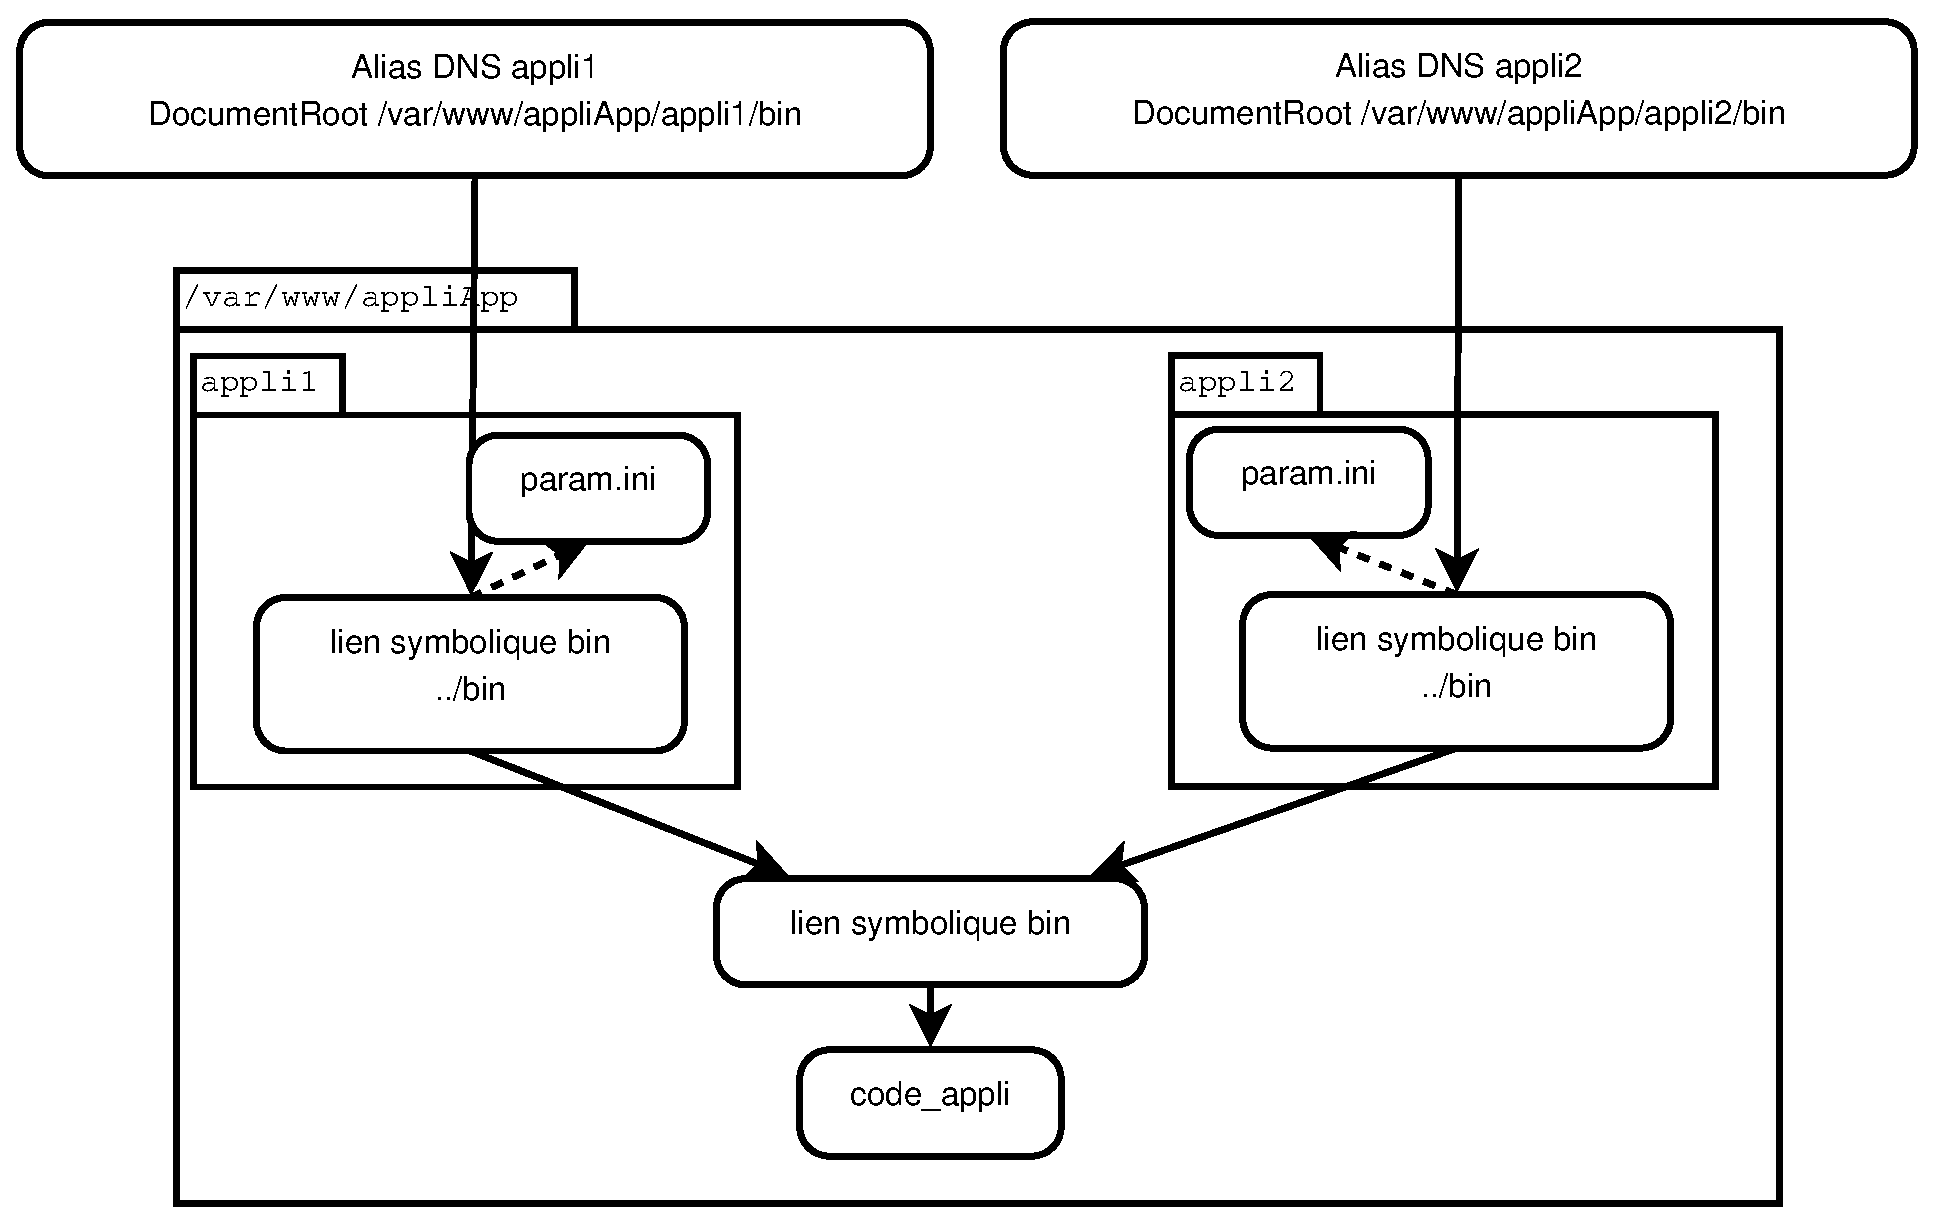
\includegraphics[width=\linewidth]{images/dnsmultiple}
\caption{\label{dnsmultipleschema}Schéma général d’implémentation pour utiliser le même code avec des noms d’application et des jeux de données différents}
\end{figure}

Dans le paramétrage de l’alias DNS (en principe, dans \textit{/etc/apache2/sites-available}), l’application pointe vers le dossier \textit{/var/www/appliApp/appli1/bin}. \textit{/var/www} correspond à la racine du site web, \textit{appliApp} au dossier racine de l’application, \textit{appli1} au dossier spécifique de l’alias DNS. Ce dossier \textit{appli1} ne contient que deux fichiers : \textit{param.ini}, qui contient les paramètres spécifiques, et \textit{bin}, qui est un lien symbolique vers le dossier \textit{../bin}.

Le dossier \textit{../bin} (donc, dans\textit{ /var/www/appliApp}) est lui aussi un alias qui pointe vers le code réel de l’application, ici \textit{code\_appli}. Le fichier \textit{param.inc.php} doit contenir les commandes suivantes pour que le fichier \textit{param.ini} soit correctement chargé selon le contexte :
\begin{lstlisting}
$chemin = substr($_SERVER["DOCUMENT_ROOT"],0, strpos($_SERVER["DOCUMENT_ROOT"],"/bin"));
$paramIniFile = "$chemin/param.ini";
\end{lstlisting}

Le fichier \textit{param.ini} sera cherché dans le dossier parent du code de l’application, c’est à dire soit dans \textit{appli1}, soit dans \textit{appli2} dans cet exemple. Il suffit qu’il contienne les paramètres adéquats pour rendre l’application utilisable dans des contextes différents à partir du même code initial.

Le fichier \textit{param.ini} est le dernier qui est traité par l'application pour récupérer les paramètres. Ceux-ci sont lus dans l'ordre suivant :

\textbf{param/param.default.inc.php $\rightarrow$ param/param.inc.php $\rightarrow$ ../param.ini}

\textit{param.ini} contiendra les entrées spécifiques liées au DNS utilisé pour accéder à l'application, en principe tout ou partie de celles-ci :
\begin{lstlisting}
APPLI_titre="Gestion des otolithes d'EABX"
BDD_schema=col, public, gacl
BDD_login=compte_de_connexion
BDD_passwd=mot_de_passe_de_connexion
BDD_dsn=pgsql:host=serveur;dbname=base_de_donnees;sslmode=require
GACL_aco=col
APPLI_code=proto
\end{lstlisting}

Si un libellé contient une apostrophe, la chaîne doit être insérée dans des guillemets doubles, comme ici pour la variable \textit{APPLI\_titre}.


\subsection{Droits à attribuer au serveur web}
\label{droitsApache}
Le serveur web doit pouvoir accéder en lecture à l'ensemble des fichiers de l'application, et en écriture à deux dossiers :
\begin{itemize}
\item \textit{display/templates\_c} : fichier utilisé par Smarty pour compiler les modèles de documents HTML ;
\item \textit{img} : dossier de génération des images et des fichiers temporaires.
\end{itemize}

Deux scripts sont fournis pour attribuer les droits : 
\begin{itemize}
\item \textbf{install/apache2/upgrade\_rights.sh} : positionne les droits en utilisant les droits standards Linux (owner, group)
\item \textbf{install/apache2/upgrade\_rights\_with\_acl.sh} : positionne les droits à partir des ACL.
\end{itemize}

Les scripts doivent être lancés ainsi :
\begin{lstlisting}
collec-2.0/install/apache2/upgrade_rights.sh v2.0
\end{lstlisting}
ou 
\begin{lstlisting}
collec-2.0/install/apache2/upgrade_rights_with_acl.sh v2.0
\end{lstlisting}


\section{Configurer l'application}

L'application est configurable par l'intermédiaire de trois fichiers :

\textbf{param/param.default.inc.php $\rightarrow$ param/param.inc.php $\rightarrow$ ../param.ini}

Le premier fichier contient les paramètres par défaut. Il est systématiquement fourni à chaque nouvelle version de l'application.

Le second est spécifique de l'implémentation. Il comprend notamment les informations liées à la connexion à la base de données, à la méthode d'identification, ou à la recherche des attributs dans l'annuaire LDAP. 

le troisième est destiné à offrir la possibilité d'accéder, à partir du même code applicatif, à plusieurs bases de données différentes (\textit{cf.} \ref{dnsmultiple} \textit{\nameref{dnsmultiple}}, page \pageref{dnsmultiple}).

Voici les principaux paramètres utilisés :

\subsection{Connexion à la base de données}

Dans la pratique, deux connexions sont nécessaires : l'une pour accéder à la base des droits, l'autre aux données proprement dites. Voici les paramètres à définir :

\begin{longtable}{|p{4cm}|p{11cm}|}
\hline
\textbf{Variable} & \textbf{Signification} \\
\hline
\endhead
BDD\_login & compte de connexion à la base de données \\
\hline
BDD\_passwd & mot de passe associé\\
\hline
BDD\_dsn & adresse de la base de données sous forme normalisée\\
\hline
BDD\_schema & schéma utilisé (plusieurs schémas peuvent être décrits, en les séparant par une virgule - fonctionnement propre à Postgresql)\\
\hline
GACL\_dblogin & compte de connexion à la base de données des droits\\
\hline
GACL\_dbpasswd & mot de passe associé\\
\hline
GACL\_dsn & adresse normalisée \\
\hline
GACL\_schema & schéma utilisé\\
\hline
GACL\_aco & nom du code de l'application utilisé dans la gestion des droits\\
\hline
\caption{Variables utilisées pour paramétrer les connexions}
\end{longtable}

\subsection{Identification des utilisateurs}

\begin{longtable}{|p{6cm}|p{10cm}|}
\hline
\textbf{Variable} & \textbf{Signification} \\
\hline
\endhead
ident\_type & Type d'identification supporté. L'application peut gérer \textbf{BDD} (uniquement en base de données),\textbf{LDAP} (uniquement à partir d'un annuaire LDAP) \textbf{LDAP-BDD} (d'abord identification en annuaire LDAP, puis en base de données), \textbf{CAS} (serveur d'identification \textit{Common Access Service}\footnote{serveur externe gérant l'identification des utilisateurs, et renvoyant à l'application le login utilisé}), et enfin \textbf{HEADER} (identification derrière un proxy qui fournit le login dans une variable d'entête HTTP)\\
\hline
CAS\_plugin & Nom du plugin utilisé pour une connexion CAS \\
\hline
CAS\_address & Adresse du serveur CAS\\
\hline
CAS\_port & Systématiquement 443 (connexion chiffrée)\\
\hline
LDAP & tableau contenant tous les paramètres nécessaires pour une identification LDAP \\
\hline
ident\_header\_login\_var & par défaut, AUTH\_USER. Nom de la variable qui contiendra le login dans le cas d'une identification en mode HEADER (le radical HTTP\_  ne doit pas être indiqué) \\
\hline
privateKey & clé privée utilisée pour générer les jetons d'identification (ré-identification automatique après une première connexion) \\
\hline
pubKey & clé publique utilisée pour générer les jetons d'identification \\
\hline
tokenIdentityValidity & durée de validité, en secondes, des jetons d'identification\\
\hline
MAIL\_enabled & Si à 1, l'envoi de mail est géré par l'application \\
\hline
CONNEXION\_max\_attemps & nombre maximum d'essais de connexion avant blocage temporaire du compte \\
\hline
CONNEXION\_blocking\_duration & durée de blocage du compte \\
\hline
APPLI\_mailToAdminPeriod & intervalle de temps entre l'envoi d'un mail de notification de blocage de compte à un administrateur \\
\hline
APPLI\_admin\_ttl & durée de vie d'une session d'administration (temps maximum entre deux accès à une page d'administration avant réidentification) \\
\hline
APPLI\_lostPassword & Si à 1, autorise la récupération du mot de passe perdu, par envoi d'un mail avec un lien chiffré. Nécessite également que MAIL\_enabled soit positionné à 1 \\
\hline

\caption{Variables utilisées pour paramétrer l'identification}
\end{longtable}

\subsubsection{Ré-identification par jeton}

L'application permet de conserver l'identification plus longtemps que celle définie dans le serveur, en rejouant la connexion avec un jeton d'identification chiffré. Cela évite, par exemple, de devoir se ré-identifier toutes les heures si on accède au logiciel à partir d'un terminal mobile (smartphone ou tablette, par exemple).

Les trois dernières variables permettent de configurer ce mode d'identification. 

Le framework peut générer un jeton chiffré après la première identification, qui sera analysé pour savoir si l'utilisateur peut être ré-identifié automatiquement.

Pour que ce mécanisme fonctionne, il faut :
\begin{itemize}
\item que le paramètre \textit{tokenIdentityValidity} ait une durée de validité supérieure à la durée de vie de la session. Il est raisonnable de ne pas fixer une durée de vie supérieure à une journée de travail (10 heures). Le cookie transmis est protégé ;
\item que les clés privée et publique, utilisées pour le chiffrement du jeton, soient accessibles au serveur web (variables \textit{privateKey} et \textit{publicKey}).
\end{itemize}

Les clés sont générées automatiquement avec le script d'installation automatique du serveur et de l'application.

Le jeton est chiffré avec la clé privée, ce qui lui permet d'être lu, le cas échéant, par l'application. Il contient le login et la date d'expiration. 

Si l'utilisateur déclenche une déconnexion, le jeton est supprimé.

Pour plus d'informations, consultez comment fonctionne le mécanisme de ré-identification par jeton \cite{token}.

\subsubsection{Identification par HEADER}

Dans ce mode d'identification, le serveur web est placé derrière un serveur d'identification, appelé proxy d'identification. L'adresse de l'application pointe vers ce dernier. 

Le proxy gère la connexion de l'utilisateur, et fournit à l'application le login dans une variable configurable. Cette variable est accessible dans le tableau \$\_SERVER, par exemple \$\_SERVER [ "HTTP\_AUTH\_USER" ].

Pour activer ce mécanisme, il faut modifier les paramètres suivants dans le fichier \textit{param.ini.php} :
\begin{lstlisting}
$ident_type = "HEADER";
$ident_header_login_var = "AUTH_USER";
\end{lstlisting}

la variable ne doit pas contenir la racine HTTP\_ (une fonction l'extrait automatiquement).

\subsection{Configuration de l'accès à l'annuaire LDAP}

Les paramètres LDAP sont stockés dans un tableau :
\begin{lstlisting}
$LDAP = array(
		"address"=>"localhost",
		"port" => 389,
		"rdn" => "cn=manager,dc=example,dc=com",
		"basedn" => "ou=people,ou=example,o=societe,c=fr",
		"user_attrib" => "uid",
		"v3" => true,
		"tls" => false,
		"groupSupport"=>true,
		"groupAttrib"=>"supannentiteaffectation",
		"commonNameAttrib"=>"displayname",
		"mailAttrib"=>"mail",
		'attributgroupname' => "cn",
		'attributloginname' => "memberuid",
		'basedngroup' => 'ou=example,o=societe,c=fr'
);
\end{lstlisting}


L'application peut non seulement identifier les utilisateurs auprès de l'annuaire LDAP, mais également récupérer les groupes auxquels ils appartiennent dans celui-ci.

Voici les paramètres à indiquer dans ce cas de figure (valable en principe pour tout annuaire compatible OpenLdap) : 
\begin{longtable}{|p{4cm}|p{11cm}|}
\hline
\textbf{Variable} & \textbf{Signification} \\
\hline
\endhead
address &  adresse de l'annuaire\\
\hline
port & 389 en mode non chiffré, 636 en mode chiffré\\
\hline
rdn & compte de connexion, si nécessaire \\
\hline
basedn & base de recherche des utilisateurs\\
\hline
user\_attrib & nom du champ contenant le login à tester\\
\hline
v3 & toujours à \textit{true}\\
\hline
tls & \textit{true} en mode chiffré\\
\hline
groupSupport & \textbf{true} si l'application recherche les groupes d'appartenance du login dans l'annuaire\\
\hline
groupAttrib & Nom de l'attribut contenant la liste des groupes d'appartenance\\
\hline
commonNameAttrib & Nom de l'attribut contenant le nom de l'utilisateur\\
\hline
mailAttrib & Nom de l'attribut contenant l'adresse mail de l'utilisateur\\
\hline
attributgroupname & Attribut contenant le nom du groupe lors de la recherche des groupes (cn par défaut)\\
\hline
attributloginname & attribut contenant les membres d'un groupe\\
\hline
basedngroup & base de recherche des groupes \\
\hline
\caption{Variables utilisées pour paramétrer l'accès à l'annuaire LDAP}
\end{longtable}

\subsection{Paramètres spécifiques}
\label{paramspec}

\begin{longtable}{|p{4cm}|p{11cm}|}
\hline
\textbf{Variable} & \textbf{Signification} \\
\hline
\endhead
APPLI\_photoStockage & dossier contenant les photos générées par l'application, avant transmission au navigateur. Par défaut : \textit{img}\\
\hline
APPLI\_maxfilesize & Taille maximale des photos téléchargeables. Par défaut : 100000000 \\
\hline

\caption{Variables spécifiques}
\end{longtable}

\subsection{Paramètres stockés en base de données}
\label{paramdb}

À partir de la version 2, certains paramètres peuvent être stockés dans la base de données, pour éviter qu'ils ne soient dépendants de la configuration du serveur.

Ces paramètres sont accessibles depuis le menu \textit{administration}, item \textit{Paramètres de l'application}.

Voici la liste des paramètres actuellement décrits :
\begin{longtable}{|p{4cm}|p{11cm}|}
\hline
\textbf{Variable} & \textbf{Signification} \\
\hline
\endhead
APPLI\_title & Titre de l'application tel qu'il figure entre l'icône et le menu\\
\hline
\caption{Paramètres stockés dans la base de données}
\end{longtable}


\section{Créer la base de données}

La base de données est composée de deux schémas : l'un pour stocker les informations d'identification, les droits d'accès et les traces, l'autre pour les données proprement dites.

Le schéma \textit{public} ne devrait jamais être utilisé pour stocker l'information : réservez-le pour les composants communs, comme Postgis.

Les tables de gestion des droits peuvent être communes à plusieurs jeux / applications différentes : la variable \textit{GACL\_aco} permet de séparer la gestion des droits pour chaque application, tout en travaillant à partir des mêmes utilisateurs (répartis le cas échéant dans des groupes différents selon le jeu de données considéré).

Les scripts de création des schémas dans la base de données sont stockés dans le dossier \textit{install/pgsql}. 



\subsection{Créer les tables de gestion des droits}
Script à utiliser : \textit{gacl\_create\_2.0.sql}. Les tables nécessaires vont être créées dans le schéma \textit{gacl} (ne modifiez pas le nom du schéma).

Le script crée un compte d'administration par défaut :
\begin{itemize}
\item login : \textbf{admin}
\item mot de passe : \textbf{password}
\end{itemize}

Il devra être supprimé quand un autre compte d'administration aura été créé.


\subsection{Créer les tables applicatives}
Script à utiliser : \textit{otolithe\_create-2.0.sql}.

Par défaut, le script crée un schéma appelé \textit{otolithe}. Il est possible de créer plusieurs schémas différents, si l'application supporte plusieurs jeux de données (\textit{cf.} \ref{dnsmultiple} \textit{\nameref{dnsmultiple}}, page \pageref{dnsmultiple}). Dans ce cas de figure, remplacez \textit{otolithe} par le nom du schéma voulu dans les deux premières lignes du script.

\subsection{Login de connexion}

Si la base de données et l'application sont hébergés dans deux serveurs différents, il est fortement conseillé de créer deux logins de connexion, un pour le schéma des droits, l'autre pour les schémas applicatifs. Ces logins ne doivent pouvoir être utilisés que depuis le serveur web hébergeant l'application.

Cette opération est possible en modifiant le fichier \textit{/etc/postgresql/9.5/main/pg\_hba.conf} selon ce principe :

\begin{lstlisting}
# Connexions pour les serveurs web 
host nom_database userGacl adresse_serveur/32 md5 
host nom_database userData adresse_serveur/32 md5
\end{lstlisting}

Le login utilisé dans \textit{userGacl} correspond à la variable \textit{\$GACL\_dblogin}, et \textit{userData} à \textit{\$BDD\_login}.

et en rechargeant ensuite la configuration de Postgresql avec la commande :
\begin{lstlisting}
service postgresql reload
\end{lstlisting}

\subsection{Droits sur les tables}

Le compte utilisé pour la connexion au schéma des droits doit pouvoir modifier les informations présentes dans l'ensemble des tables de \textit{gacl}. Il ne devrait pas pouvoir accéder aux autres schémas (hormis \textit{public}), sauf en cas d'installation mono-serveur (base de données hébergée dans la même machine et connexion à distance impossible).

Le compte utilisé pour accéder aux schémas des données doit pouvoir modifier l'ensemble des informations dans les schémas de données, et lire la table \textit{gacl.aclgroup}.

Le plus simple est d'utiliser le logiciel \textit{pgAdmin} \cite{pgadmin} pour attribuer les droits.

Le script d'installation automatique rend le compte \textit{otolithe} propriétaire de la base de données, ce qui simplifie la gestion des droits sur les tables.

\subsection{Scripts de modification}

Lors de la livraison de nouvelles versions, il est possible que des scripts de modification soient livrés pour mettre à niveau la base de données. Ces scripts doivent être exécutés dans tous les schémas contenant des données applicatives (pour plus de détails, consultez ci-après \textit{\nameref{newVersion}}).

\section{Mise en production}

Une fois l'application configurée, et après avoir créé un nouveau compte d'administration :
\begin{itemize}
\item supprimez le compte \textit{admin}, livré par défaut, qui ne doit pas être conservé. Sa désactivation n'est pas suffisante : si pour une raison ou pour une autre le compte est réactivé, n'importe qui pourra récupérer les droits totaux ;
\item supprimez le dossier \textit{install} qui contient les scripts de création des tables ;
\item déplacez le dossier \textit{database}, qui contient la documentation d'installation et de configuration (elle n'a pas à rester accessible depuis le site web) ;
\item faites une revue des droits, pour vous assurer que tout est correctement configuré.
\end{itemize}

Vous pouvez également tester si la configuration du serveur est correcte en recourant à \textit{ZAProxy} \cite{zaproxy}, qui analysera la communication entre le serveur et un navigateur et identifiera les problèmes éventuels de non conformité (mauvaise réécriture des entêtes HTML suite à une mauvaise configuration du serveur Apache, par exemple).

\section{Installer une nouvelle version}
\label{newVersion}
\subsection{Faites une sauvegarde de la base de données}
Il arrive fréquemment que la structure de la base de données évolue. Avant toute opération, assurez-vous de disposer d'une sauvegarde, dans un autre support.

Un programme de sauvegarde est disponible dans \textit{install/pgsql/backup.sh}. Vous pouvez l'exécuter manuellement ainsi :
\begin{lstlisting}
su postgres -c "install/pgsql/backup.sh"
\end{lstlisting}

La sauvegarde sera stockée dans \textbf{/var/lib/postgresql/backup}.

Si vous avez utilisé le script d'installation automatique, le programme est également présent dans \textit{/var/lib/postgresql}.

\subsection{Sauvegarder le fichier contenant les paramètres de l'application}

Le fichier \textit{param/param.inc.php} contient vos paramétrages spécifiques. Lors de l'installation d'une nouvelle version, il va être supprimé.

Faites-en une copie, et remettez-le en place après avoir installé la nouvelle version.

\subsection{Consultez le fichier news.txt}

Le fichier \textit{param/news.txt} contient la description des modifications apportées au logiciel. Il précise notamment si une mise à jour de la base de données doit être appliquée.

\subsection{Mise à jour de la structure de la base de données}

Le dossier \textit{install/pgsql} contient les scripts de création et de mise à jour de la base de données. Les scripts de mise à jour sont nommés ainsi :
\begin{lstlisting}
col_alter_versionAnterieure-versionMiseAJour.sql
\end{lstlisting}

\textit{versionAnterieure} correspond à la version la plus ancienne qui doit être mise à jour, \textit{versionMiseAJour} la version cible. Par exemple :
\begin{lstlisting}
otolithe_alter_2.0-2.1.sql
\end{lstlisting}
indique que toutes les versions entre \textit{2.0} et \textit{2.1} doivent être mises à jour avec le script indiqué. Si vous avez \og sauté \fg{} certaines versions du logiciel, il est possible que plusieurs scripts doivent être appliqués.

La mise à jour doit être appliquée dans tous les schémas contenant des données, notamment dans le cas où le même logiciel est utilisé pour gérer plusieurs jeux de données.

Avant d'exécuter les scripts, vérifiez leur contenu, et notamment le nom des schémas.

Ne relancez jamais l'exécution d'un script.

\subsection{Reconfigurer les droits d'accès au serveur web}

Après installation de la nouvelle version du code, n'oubliez-pas de reconfigurer les accès en lecture pour le compte utilisé pour faire fonctionner le serveur web, et en écriture pour les dossiers \textit{img} et \textit{display/templates\_c} (\textit{cf.} \ref{droitsApache} \textit{\nameref{droitsApache}}, page \pageref{droitsApache}).

\subsection{Supprimer les dossiers inutiles}
Une fois la mise en production validée, supprimez le dossier \textit{install} et déplacez le dossier \textit{database}, et faites une revue des droits pour vous assurer qu'il n'y a pas eu de modification intempestive ou que la configuration est toujours correcte.

\subsection{Vérifier la configuration du chiffrement}
Avec un navigateur récent, ou en testant le site (s'il est accessible depuis internet) à partir de \href{https://www.ssllabs.com/ssltest/}{SSLLABS}, vérifiez que l'application soit correctement configurée, notamment au niveau du serveur Apache.

\chapter{Administrer l'application}

\section{Gérer les droits}
\label{droits}

Depuis la version 1.1, les scripts de création des bases de données intègrent la génération initiale des groupes et des droits associés, ceci afin de faciliter la phase de mise en route.

Toutefois, vous devrez créer des groupes d'utilisateurs correspondant à vos projets, et modifier ensuite les projets pour donner les droits adéquats aux groupes créés.

\subsection{Principe général}

Les droits sont gérés selon le principe initialement utilisé dans la bibliothèque PHPGACL \cite{phpgacl}, aujourd'hui obsolète. 

Les logins sont déclarés dans des groupes organisés de manière hiérarchique : un groupe hérite des droits attribués à ses parents.

Les droits utilisés dans le logiciel sont associés à des groupes. Il est possible d'attribuer plusieurs droits à un même groupe, et un droit peut être détenu par des groupes différents.

Si le paramètre \textit{\$LDAP["groupSupport"]} est positionné à \textit{true}, les groupes dont fait partie le compte LDAP sont également récupérés. Si ces groupes se voient attribués des droits, les comptes associés les récupéreront automatiquement.

Voici le schéma des tables utilisées pour gérer les droits :

\begin{figure}[H]
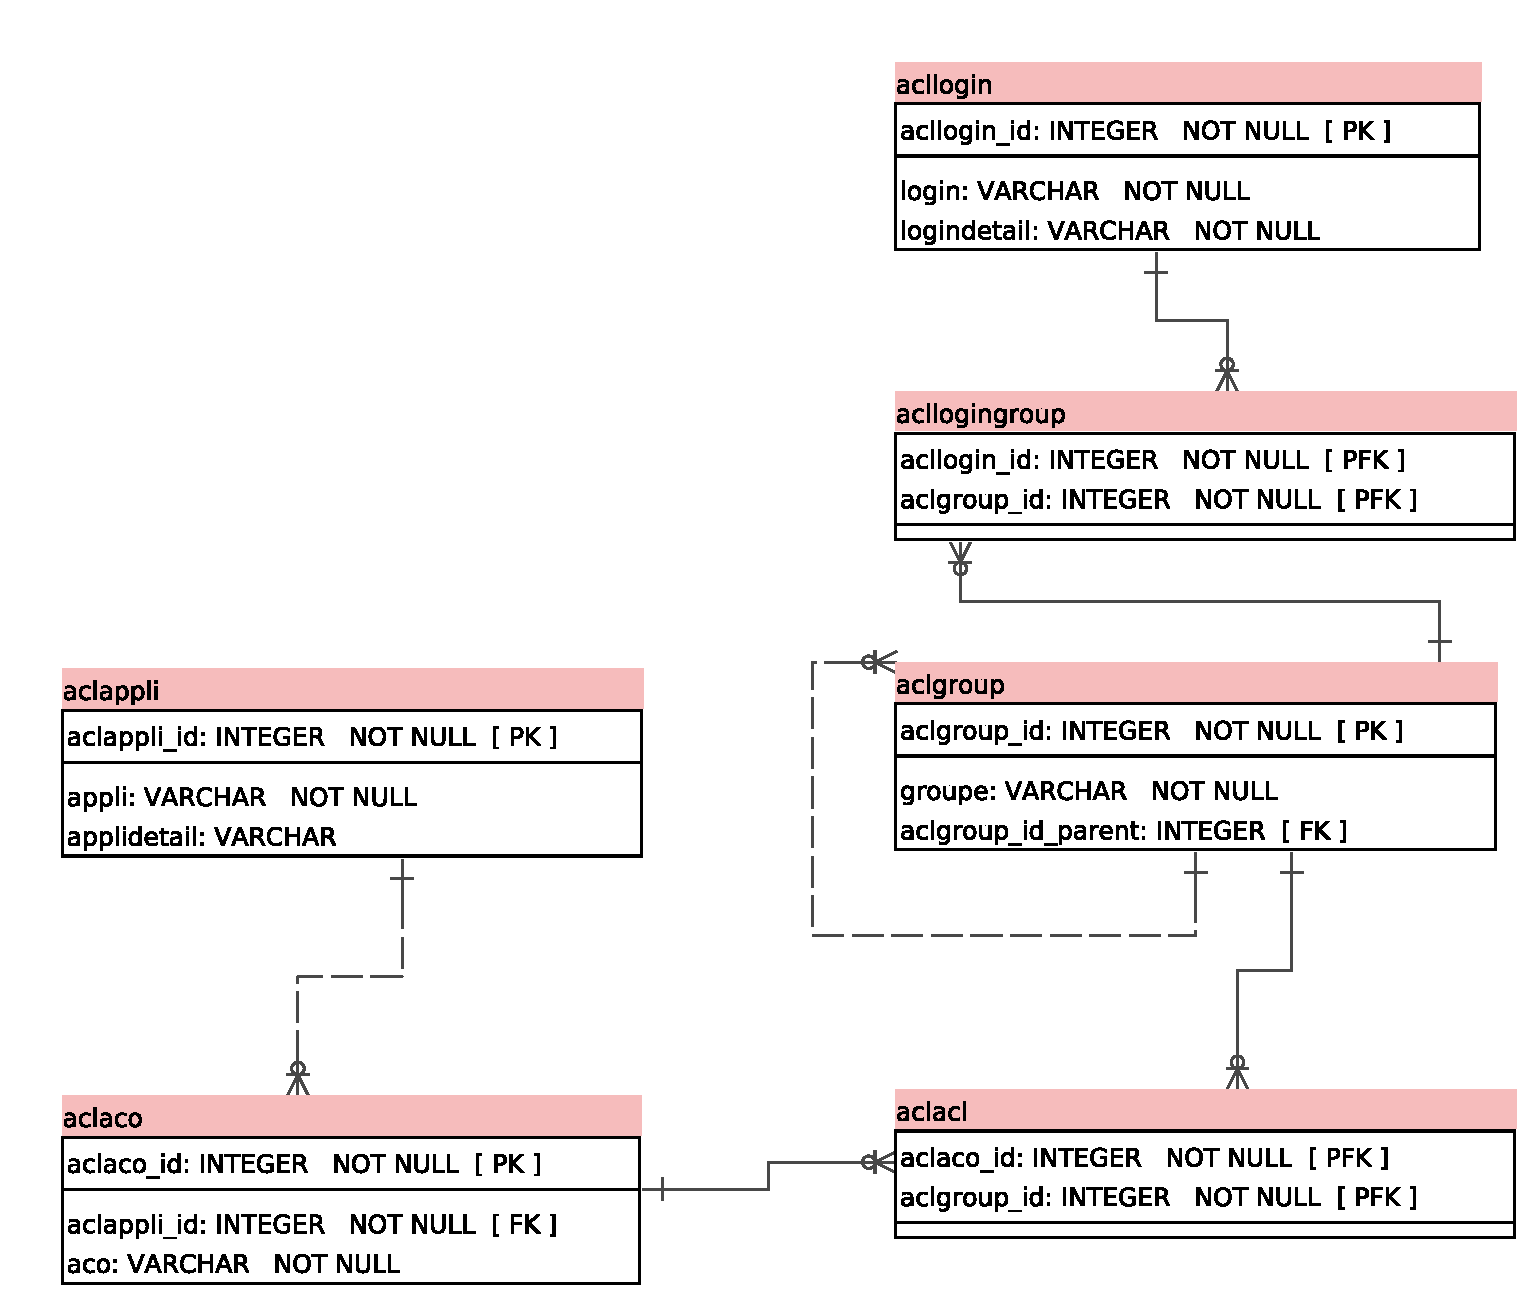
\includegraphics[width=\linewidth]{images/acl_only}
\caption{Schéma des tables utilisées pour gérer les droits}
\end{figure}

Voici la description des tables :
\begin{description}
\item[acllogin] : liste des logins utilisés. Si un compte est créé dans la base locale d'identification, un enregistrement est également créé dans cette table. Pour les identifications LDAP ou CAS, ils doivent être identiques. Si seuls les groupes LDAP sont utilisés pour un compte, il n'a pas besoin d'être décrit ici ;
\item[aclappli] : liste des applications gérées. Il est possible de gérer, à partir de la même base de données, plusieurs ensembles de droits, qui utilisent les mêmes logins.
\item[aclaco] : liste des droits déclarés dans l'application ;
\item[aclgroup] : liste des groupes contenant les logins, et qui détiennent les droits. Un groupe peut hériter d'un autre groupe. Les droits associés au groupe parent sont également attribués au groupe hérité ;
\item[acllogingroup] : table permettant de déclarer les logins associés à un groupe ;
\item[aclacl] : table décrivant les droits détenus par un groupe.
\end{description}

Le module d'administration permet de saisir toutes ces informations. Il faut que l'utilisateur dispose du droit \textit{admin}, c'est à dire qu'il fasse partie du groupe \textit{admin} (configuration par défaut à l'initialisation de la base des droits) pour pouvoir accéder à ces fonctions.

\subsection{Créer un nouvel utilisateur}

Les utilisateurs peuvent être issus soit de l'annuaire LDAP, soit de la base interne. 
Pour créer un nouvel utilisateur dans la base locale :
\begin{itemize}
\item \textit{Administration $\rightarrow$ Liste des comptes }
\item \textit{Nouveau login}
\item renseignez au minimum le login.
\end{itemize}

\begin{figure}[H]
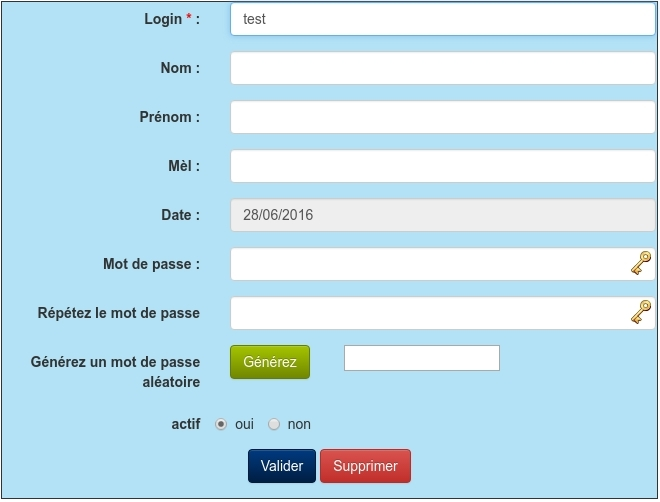
\includegraphics[width=\linewidth]{images/user_create}
\caption{Écran de saisie d'un login de connexion}
\end{figure}

Pour créer le mot de passe, vous pouvez cliquer sur le bouton \textit{Générez}, qui  en générera un automatiquement. Envoyez-le par mél à son destinataire (par \textit{copier-coller}), en lui demandant de le modifier à la première connexion (icône en forme de clé, dans le bandeau, en haut à droite).

Les mots de passe doivent respecter les règles suivantes :
\begin{itemize}
\item ils doivent avoir une longueur minimale de 8 caractères ;
\item ils doivent comprendre trois types de caractères différents parmi les minuscules, majuscules, chiffres et caractères de ponctuation ;
\item ils ne peuvent pas être réutilisés pour le même login ;
\item les mots de passe n'expirent pas.
\end{itemize}

Les mots de passe sont stockés sous forme d'empreinte, calculée en rajoutant un sel\footnote{chaîne de caractère rajoutée au mot de passe -- en général le login ou un identifiant -- qui permet d'éviter que deux mots de passe identiques, associés à deux logins différents, aient la même empreinte} et encodés en SHA256 : ils ne peuvent pas être retrouvés en cas de perte.

L'application n'intègre pas de module permettant de régénérer automatiquement un mot de passe en cas de perte : c'est au responsable applicatif d'en fournir un nouveau.

La création d'un compte entraîne la création d'une entrée identique dans la table des \textit{acllogin}, utilisée pour attribuer les droits.

Pour désactiver temporairement un compte, sélectionnez \textit{non} dans la zone \textit{actif}. Si le compte ne doit plus être utilisé, supprimez-le.

Attention : si le compte disposait des droits d'administration, assurez-vous que vous avez toujours un compte disposant des mêmes droits avant la suppression.

\subsection{Créer un login utilisé dans la gestion des droits}

Indépendamment du compte de connexion, qui peut être soit issu de la base interne, soit récupéré auprès d'un annuaire LDAP ou d'un serveur CAS, l'application a besoin de connaître les utilisateurs pour pouvoir leur attribuer des droits.

À partir du menu, choisissez \textit{Administration $\rightarrow$ ACL - logins}.

Vous pouvez modifier un login existant ou en créer un nouveau. Dans ce cas, vous devrez indiquer au minimum le login utilisé (identique à celui qui est employé pour la connexion à l'application : base de données interne, annuaire LDAP, serveur CAS).

\begin{figure}[H]
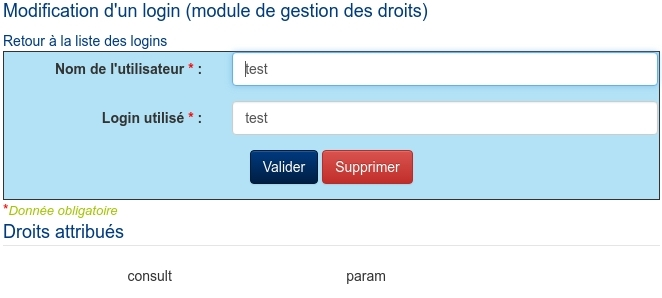
\includegraphics[width=\linewidth]{images/acl_login}
\caption{Écran de modification d'un login dans le module de gestion des droits}
\end{figure}


Sous l'écran de saisie figurent la liste des droits attribués à un login (en modification, le calcul n'est réalisé qu'à l'affichage de la page).

\subsection{Définir les groupes d'utilisateur}

Les groupes d'utilisateurs sont gérés selon un mécanisme d'héritage. Un groupe de haut niveau hérite des groupes précédents : si des droits ont été attribués à un groupe de niveau inférieur, un login associé à un groupe de niveau supérieur les récupère également.

Pour définir les groupes, dans le menu, choisissez \textit{Administration $\rightarrow$ ACL - groupes de logins}.

\begin{figure}[H]
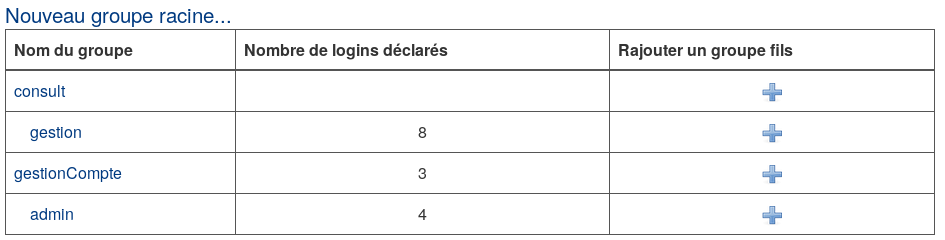
\includegraphics[width=\linewidth]{images/acl_groupe.png}
\caption{Liste des groupes de logins}
\end{figure}

Ainsi, le login déclaré dans le groupe \textit{admin} récupérera les droits attribués aux groupes \textit{gestionCompte}.

Pour créer un groupe, il existe deux possibilités :
\begin{itemize}
\item soit le groupe est à la base d'une nouvelle branche : utilisez alors \textit{Nouveau groupe racine...} ;
\item soit le groupe hérite d'un autre groupe : cliquez sur le signe + (\textit{Rajouter un groupe fils}).
\end{itemize}

Vous pouvez indiquer les logins qui sont rattachés à ce groupe.


\subsection{Créer une application}
Le moteur utilisé pour faire fonctionner le logiciel Otolithe permet de gérer des droits différents pour des jeux de données différents, à partir du même code applicatif. Chaque couple \textit{logiciel} $\leftrightarrow$ \textit{base de données} constitue donc une \textit{application}, au sens de la gestion des droits.

Il est ainsi possible, à partir de la même base de données, de définir des droits différents selon les jeux de données utilisés (un jeu de données correspond à un schéma de base de données comprenant l'intégralité des tables applicatives).

À partir du menu, choisissez \textit{Administration $\rightarrow$ ACL - droits} :

\begin{figure}[H]
\centering
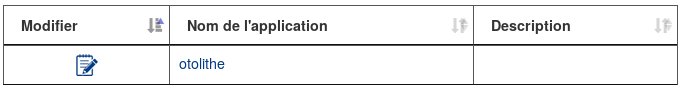
\includegraphics[width=0.7\linewidth]{images/liste_appli.png}
\caption{Liste des applications déclarées}
\end{figure}

Pour créer une nouvelle application, choisissez \textit{Nouvelle application...}. 

\begin{figure}[H]
\centering
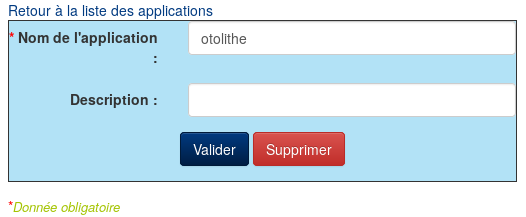
\includegraphics[width=0.7\linewidth]{images/appli_change.png}
\caption{Écran de saisie d'une application}
\end{figure}

Le nom de l'application doit impérativement correspondre à la valeur \textit{\$GACL\_appli} dans les fichiers de paramètres : c'est ce qui permet au framework de savoir quels droits appliquer.

\subsection{Définir les droits utilisables dans l'application}

À partir de la liste des applications, cliquez sur le nom de celle pour laquelle vous voulez définir les droits utilisables. 
À partir de la liste, sélectionnez \textit{Nouveau droit...}.

\begin{figure}[H]
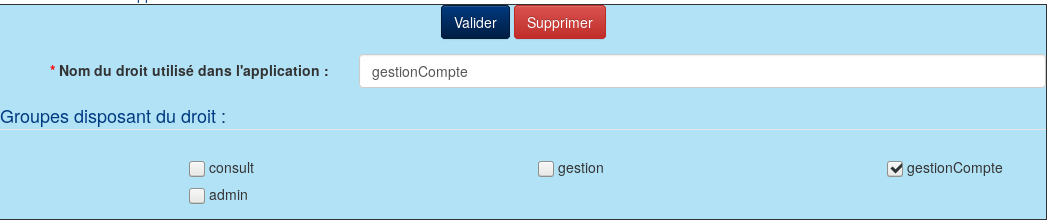
\includegraphics[width=\linewidth]{images/appli_droit.png}
\caption{Écran de saisie des droits associés à une application}
\label{applidroit}
\end{figure}

Le nom du droit doit être celui défini dans le corps de l'application (les droits sont positionnés dans les fichiers \textit{param/actions.xml}, qui contient la liste des modules utilisables, et \textit{param/menu.xml}, qui sert à générer le menu -- \textit{cf.} table \ref{droitsCollec} \textit{\nameref{droitsCollec}}, page \pageref{droitsCollec}).

Indiquez les groupes d'utilisateurs qui seront associés au droit courant.

\subsection{Cas particulier des groupes et des logins issus d'un annuaire LDAP}

Si vous avez paramétré l'application pour qu'elle s'appuie sur un annuaire LDAP pour gérer l'affectation des utilisateurs dans les groupes, vous n'êtes pas obligés de les déclarer explicitement dans le module de gestion des droits.

\subsubsection{Droits attribués à un groupe LDAP}

Tous les utilisateurs d'un groupe héritent d'un droit dans l'application.

\begin{itemize}
\item définissez le nom du groupe (en respectant la casse) dans le tableau des groupes d'utilisateurs (par exemple, EABX) ;
\item sélectionnez le nom de ce groupe dans les droits utilisables ;
\item tous les utilisateurs de l'annuaire LDAP récupéreront automatiquement les droits attribués à ce groupe.
\end{itemize}

\subsubsection{Droits attribués à un utilisateur particulier de l'annuaire LDAP}

Un utilisateur s'identifie auprès de l'annuaire LDAP, mais dispose de droits particuliers.

\begin{itemize}
\item créez son login dans la gestion des droits ;
\item rajoutez-le dans le groupe d'utilisateurs adéquat.
\end{itemize}


\section{Droits spécifiques de l'application Otolithe}

\subsection{Droits à positionner}
Voici les droits nécessaires pour faire fonctionner correctement l'application :

\begin{longtable}{|p{5cm}|p{10cm}|}
\hline
\textbf{Droit} & \textbf{Usage} \\
\hline
\endhead
admin &	Gestion des utilisateurs et des droits\\
\hline
gestionCompte &	Ajout d'un utilisateur (lecteur), création d'une expérimentation, rattachement d'un lecteur à une expérimentation, importation de poissons dans une expérimentation, suppression d'une lecture\\
\hline
gestion &	Ajout d'un poisson dans une expérimentation, de photos, etc. \\
\hline
consult	& Droit technique, permettant la consultation des informations générales, sans possibilité de modification. Les lecteurs disposent de ce droit\\
\hline
lecteur & Réalisation d'une lecture d'une photo, avec possibilité de supprimer ses propres lectures. Droit attribué par défaut à tout lecteur. C'est un droit qui est positionné automatiquement par le logiciel dès lors que le lecteur a été enregistré \\
\hline


\caption{\label{droitsCollec}Liste des droits utilisés}
\end{longtable}

Ces droits doivent être définis pour chaque application (couple \textit{logiciel} $\leftrightarrow$ \textit{base de données}) gérée par la base de gestion des droits.

\section{Gestion des traces}

Tous les appels lancés par les utilisateurs vers les modules de l'application sont enregistrés dans la table \textit{gacl.log}, qui ne doit être accessible qu'aux personnes dûment autorisées. Les traces sont supprimées au bout d'un an (script de nettoyage exécuté lors de la connexion d'un utilisateur).

Voici un exemple de trace générée :
\begin{lstlisting}
log_id	login	nom_module	log_date	commentaire	ipaddress
log_id	login	nom_module	log_date	commentaire	ipaddress
5349	eric.quinton	otolithe-photoGetPhoto	2018-08-27 11:17:29	ok	10.33.64.101
5347	eric.quinton	otolithe-photolectureSwap	2018-08-27 11:17:26	ok	10.33.64.101
5348	eric.quinton	otolithe-photolectureDisplay	2018-08-27 11:17:26	ok	10.33.64.101
5346	eric.quinton	otolithe-photoGetThumbnail	2018-08-27 11:17:18	ok	10.33.64.101
5345	eric.quinton	otolithe-photoDisplay	2018-08-27 11:17:17	ok	10.33.64.101
5344	eric.quinton	otolithe-photoGetThumbnail	2018-08-27 11:17:14	ok	10.33.64.101
5343	eric.quinton	otolithe-pieceDisplay	2018-08-27 11:17:13	ok	10.33.64.101

\end{lstlisting}

La colonne \textit{commentaire} précise des informations concernant soit la connexion, soit l'écriture en base de données : dans ce cas, l'identifiant considéré est indiqué.
L'adresse IP est en principe celle de l'utilisateur, y compris en prenant en compte le passage par un serveur Reverse-proxy\footnote{serveur mis en entrée du réseau privé, qui permet de masquer les adresses internes et de contrôler les accès depuis Internet}.

Parallèlement, les messages d'erreur sont envoyés au processus Linux SYSLOG, qui enregistre les traces dans le fichier \textit{/var/log/apache2/error.log}.

\chapter{Paramétrer le logiciel}
\section{Créer les lecteurs}
La liste des lecteurs peut être consultée depuis le menu \textit{Administration}  $\rightarrow$ \textit{Lecteurs}. 

\begin{figure}[H]
\centering
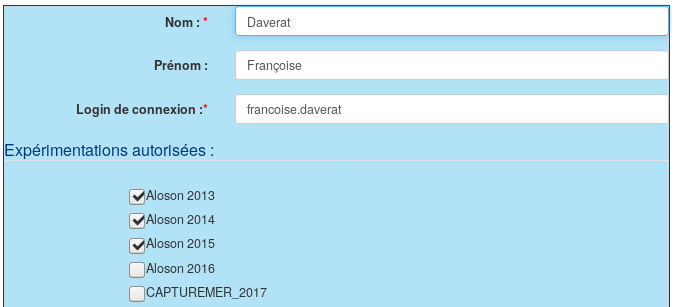
\includegraphics[width=0.7\linewidth]{images/lecteurs}
\caption{Détail d'un lecteur}
\end{figure}

Les informations à indiquer pour chaque lecteur sont les suivantes :
\begin{itemize}
\item son nom (obligatoire)
\item son prénom
\item son login de connexion (issu de la base de données interne ou de l'annuaire LDAP, le cas échéant)
\end{itemize}

Il suffit de cocher les expérimentations auxquelles il aura droit pour lui permettre de réaliser des lectures.


\section{Créer une expérimentation}
Les expérimentations sont les éléments de base de l'application. Elles sont utilisées pour gérer les droits attribués aux lecteurs.

Pour créer une expérimentation, choisissez \textit{Paramètres}  $\rightarrow$ \textit{Expérimentations}. Vous pouvez modifier une expérimentation existante ou en créer une nouvelle.

\begin{figure}[H]
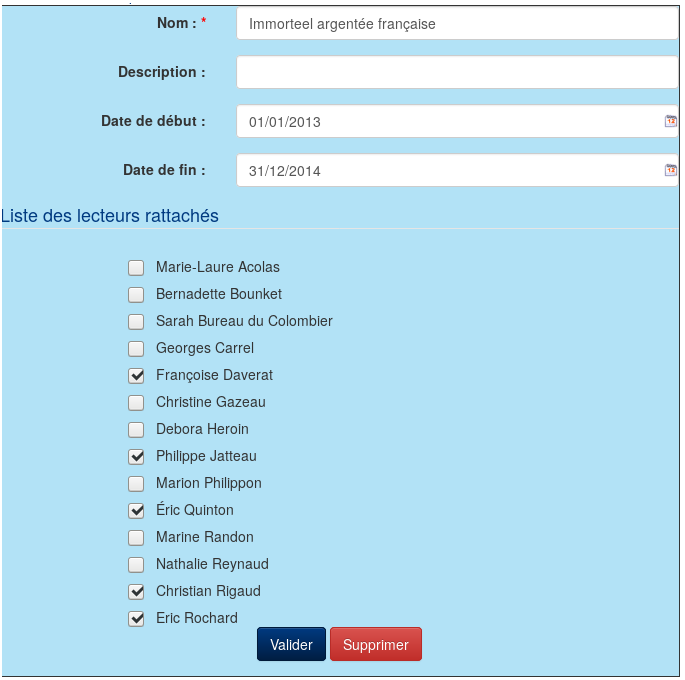
\includegraphics[width=\linewidth]{images/experimentation}
\caption{Écran de saisie/modification d'une expérimentation}
\end{figure}

La liste des lecteurs potentiels est affichée, il suffit de sélectionner ceux qui seront retenus pour lire les photos de l'expérimentation considérée.

À noter que seul le nom de l'expérimentation est obligatoire.

\section{Importer des poissons et des pièces calcifiées}

Pour éviter une saisie qui peut être fastidieuse, le logiciel permet d'importer un lot de poissons et leurs pièces calcifiées associées. L'importation automatique des photos n'est par contre pas possible.

Pour importer des poissons, choisissez \textit{Lectures} $\rightarrow$ \textit{Import}. 

\begin{figure}[H]
\centering
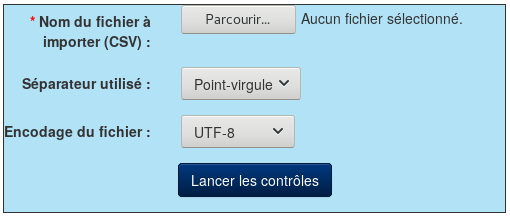
\includegraphics[width=0.7\linewidth]{images/import}
\caption{Écran de gestion des importations de poisson}
\end{figure}

L'importation est réalisée en deux étapes. Pendant la première, la conformité du fichier est vérifiée : si des anomalies sont détectées, elles sont affichées.

Si aucune anomalie n'est détectée, l'importation peut être déclenchée.

Voici la liste des colonnes qui peuvent être utilisées :

\begin{itemize}
\item \textbf{exp\_id} : code numérique de l'expérimentation (obligatoire)
\item  \textbf{espece\_id} : code de l'espèce (obligatoire)
\item     \textbf{tag} : N° de l'étiquette posée sur le poisson (le \textit{codeindividu} ou le \textit{tag} sont obligatoires)
\item     \textbf{codeindividu} : identifiant du poisson ou hptag
\item     \textbf{sexe\_id} : sexe du poisson (1 : mâle, 2 : femelle, 3 : juvénile, 4 : indifférencié)
 \item    \textbf{longueur} : longueur du poisson (mm)
\item     \textbf{poids} : poids du poisson (g)
 \item    \textbf{remarque} : remarques concernant le poisson
\item     \textbf{parasite} : parasites éventuels rencontrés
   \item  \textbf{age} : âge du poisson
  \item   \textbf{piecetype\_id} : code du type de pièce calcifiée à analyser Consultez la liste des types de pièces
   \item  \textbf{piececode} : si le type de pièce est indiqué, vous pouvez renseigner un code spécifique attaché à la pièce
  \item   \textbf{peche\_date} : date de la pêche, au format aaaa-mm-dd ou dd/mm/aaaa
   \item  \textbf{site} : site de la pêche
  \item   \textbf{zonesite} : zone précise de la pêche (précision concernant le site)
   \item  \textbf{campagne} : campagne de pêche
  \item   \textbf{peche\_engin} : engin utilisé, sous forme textuelle
   \item  \textbf{personne} : références du pêcheur
   \item  \textbf{operateur} : références de l'opérateur ayant traité le poisson
\end{itemize}

les dernières informations (site, zonesites, etc.) sont stockées sous forme de chaîne de caractères, il n'y a pas de tables qui leur sont dédiées.

\subsection{Modèle de fichier}

Un modèle de fichier utilisable pour l'importation peut être téléchargé. Le lien figure en bas de la page web.

\section{Gérer les tables de paramètres}
Deux tables de paramètres sont accessibles depuis l'application : la table des types de pièces calcifiées et la table des espèces. 

\subsection{Table des espèces}

La liste des espèces gérées par le logiciel est accessible depuis le menu \textit{Paramètres} $\rightarrow$ \textit{Espèces}. Il est possible de modifier ou rajouter un taxon (nom latin et nom français uniquement) :

\begin{figure}[H]
\centering
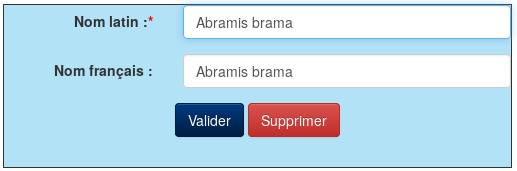
\includegraphics[width=0.5\linewidth]{images/espece}
\caption{Écran de modification d'un taxon}
\end{figure}

Le code affiché dans la liste est celui à utiliser pour les importations.

\subsection{Table des types de pièces calcifiées}

La liste des types de pièces peut être étendue depuis le menu \textit{Paramètres} $\rightarrow$ \textit{Pièces}. Seul le nom de la pièce est à indiquer.

\begin{figure}[H]
\centering
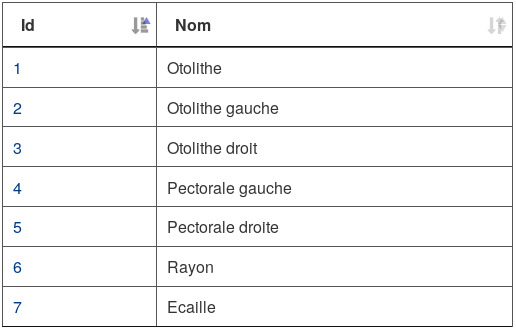
\includegraphics[width=0.5\linewidth]{images/piece}
\caption{Liste des types de pièces calcifiées}
\end{figure}

Le code affiché (colonne \textit{Id}) est celui à utiliser pour les importations.



\chapter{Gérer les lectures}
\section{Sélectionner un poisson}
Le menu \textit{Lectures} permet d'accéder à une fenêtre de recherche des poissons. 

\begin{figure}[H]
\centering
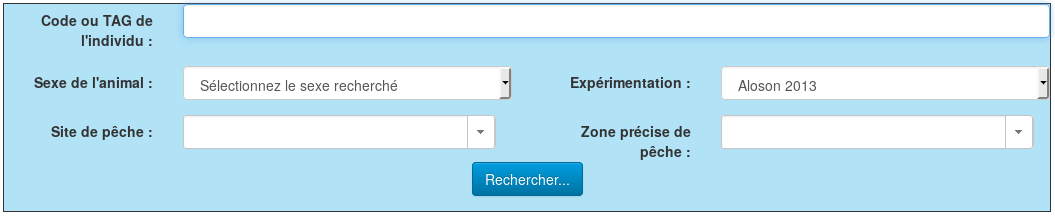
\includegraphics[width=\linewidth]{images/recherchePoisson}
\caption{Fenêtre de recherche des poissons}
\end{figure}

Seules les expérimentations pour lequel l'utilisateur dispose des droits de lecture sont affichées. Il est possible de rechercher les poissons en utilisant un des deux codes disponibles (code de l'individu ou TAG).

La sélection d'un poisson permet d'atteindre sa page de détail :
\begin{figure}[H]
\centering
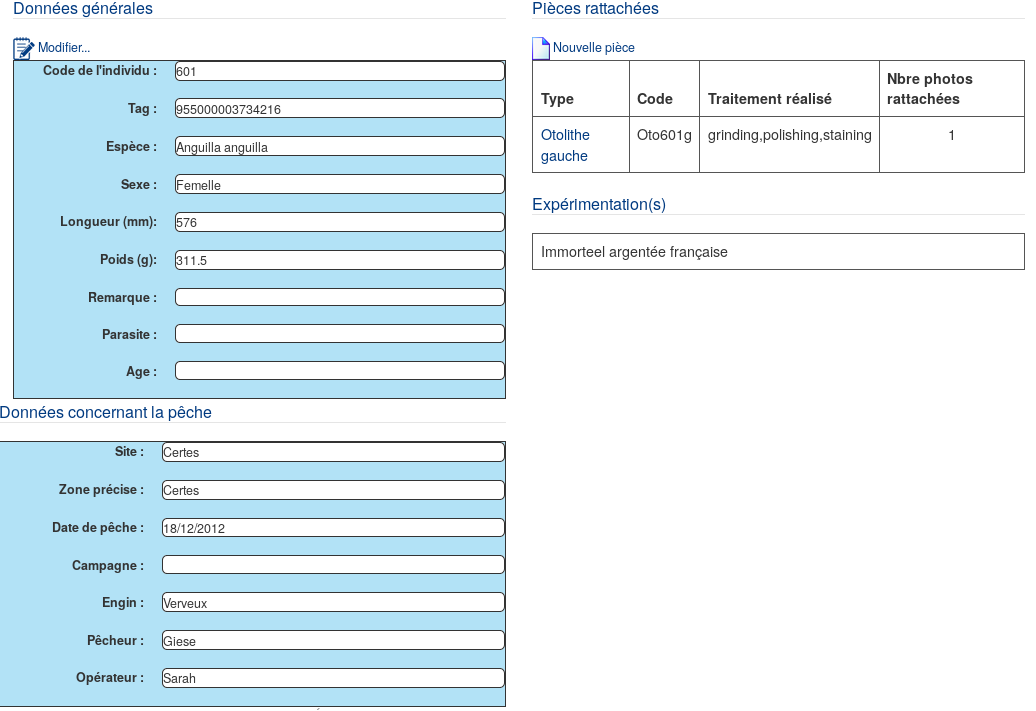
\includegraphics[width=\linewidth]{images/poissonDetail}
\caption{Fenêtre de détail d'un poisson}
\end{figure}

\subsection{Modifier un poisson}

Si les droits sont suffisants, l'utilisateur peut modifier les informations concernant un poisson. 

\begin{figure}[H]
\centering
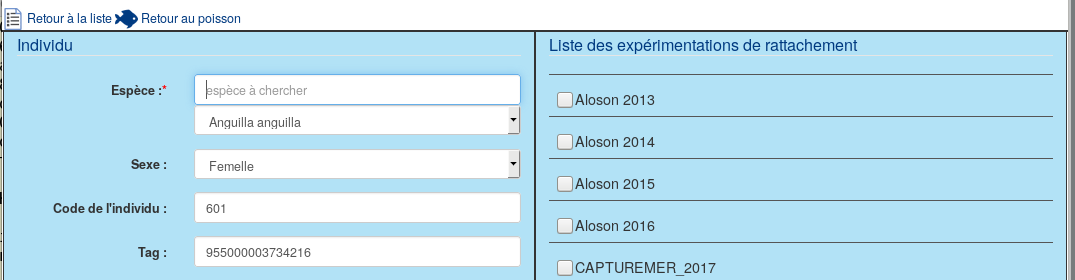
\includegraphics[width=\linewidth]{images/poissonModif}
\caption{Fenêtre de modification d'un poisson}
\end{figure}

La sélection de l'espèce se fait en tapant quelques caractères de l'espèces à chercher (nom latin ou français), puis en sélectionnant dans la liste déroulant l'information pertinente.

À noter que cet écran permet de l'associer avec une ou plusieurs expérimentations (au moins une à sélectionner -- ne pas supprimer l'expérimentation initiale sous peine de \og perdre \fg{} le poisson et de ne pas pouvoir le retrouver par l'application).

\subsection{Ajouter des pièces calcifiées}

Si elles n'ont pas été créées lors de l'importation, les pièces calcifiées peuvent être rajoutées manuellement. Seul le type de la pièce est obligatoire.

\section{Gestion des photos}

L'ajout d'une photo n'est possible que depuis le détail d'une pièce calcifiée. Il est possible d'en ajouter autant que nécessaire pour la même pièce, mais la lecture n'est réalisable que photo par photo.

\subsection{Limitations quant au format et aux dimensions d'une photo}

Si le format TIFF est souvent plébiscité pour son absence de perte d'informations, il présente l'inconvénient de ne pas être supporté par les navigateurs et ne peut pas être utilisé pour réaliser les lectures. De plus, il est assez gourmand en espace de stockage.

Le logiciel autorise toutefois l'importation de photos au format TIFF, sachant que celles-ci seront transformées en JPG au moment de la lecture (le format d'origine est conservé dans la base de données).

Les logiciels associés aux microscopes peuvent générer des photos au format TIFF mal formées (messages d'erreur lors de leur ouverture). Si une photo n'arrive pas à être importée, il convient de l'ouvrir avec le logiciel GIMP \cite{gimp}, puis l'enregistrer de nouveau : les messages d'erreur seront supprimés lors de cette étape. Ce logiciel est également très efficace pour réduire la taille d'une photo trop volumineuse.

Pour des raisons de performance, il est déconseillé d'importer des photos de plus de 50 Mo, celles-ci étant retraitées par le serveur avant d'être stockées.

Les photos sont stockées dans la base de données dans leur format original et sous forme de miniature, pour réduire les temps de traitement.

\subsection{Repère de mesure et longueur de référence}

Il est courant d'insérer un repère de mesure sur une photo. En connaissant sa longueur en pixels (dans la photo d'origine), il est alors facile de calculer des distances sur la photo, et notamment les écartements entre les points lors de la lecture.

Si ces deux informations sont renseignées, les lecteurs n'auront pas besoin de mesurer individuellement la taille de la longueur de référence pour recalculer les dimensions mesurées sur la photo.

\section{Gestion des lectures}

Il est possible de réaliser autant de lectures que nécessaire, celles-ci étant datées.

Pour des questions de performances, la taille de la photo transmise au navigateur peut volontairement être réduite. Les résolutions par défaut proposées sont les suivantes :
\begin{itemize}
\item 800x600
\item 1024x768
\item 1280x1024
\item 1600x1300
\item taille originale
\end{itemize}

Les lecteurs peuvent choisir la résolution qui leur convient le mieux, sachant que plus la photo est détaillée, plus elle est volumineuse. 

Le placement des points sur la photo est recalculé en tenant compte du facteur de réduction : le logiciel permet ainsi de visualiser l'ensemble des lectures effectuées quelle que soit la résolution utilisée par chaque lecteur.

\subsection{Tableau des lectures}

\begin{figure}[H]
\centering
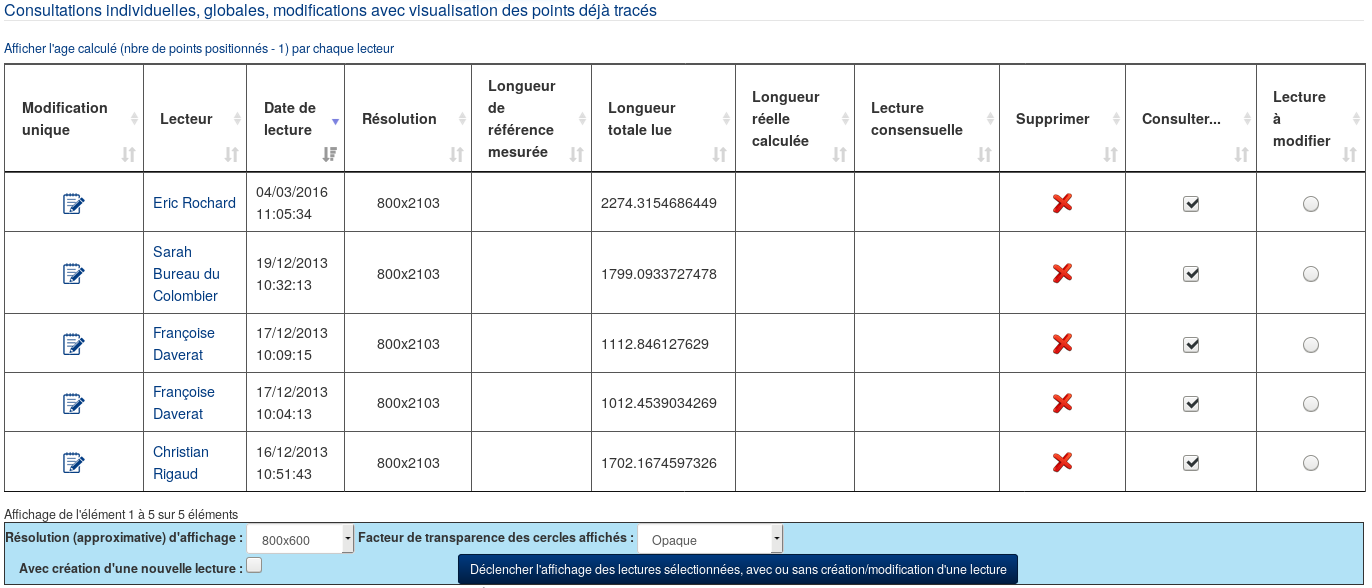
\includegraphics[width=\linewidth]{images/lectureTableau}
\caption{Tableau récapitulatif des lectures réalisés sur une photo}
\end{figure}

Le tableau des lectures permet de consulter l'ensemble des lectures réalisées, soit individuellement, soit globalement. Le formulaire en bas de tableau permet ainsi de créer une nouvelle lecture en affichant celles qui sont sélectionnées, par exemple pour créer une lecture consensuelle.

Par défaut, pour ne pas influencer les lecteurs, le nombre de segments déterminés par les lecteurs précédents n'est pas affiché. Il suffit de cliquer sur le lien \textit{Afficher l'age calculé (nbre de points positionnés - 1) par chaque lecteur} pour obtenir le nombre de segments identifiés.

Pour faciliter la visualisation des points sur les photos, il est possible d'ajuster leur facteur de transparence, depuis opaque jusqu'à totalement transparent.

\subsection{Réaliser une lecture}

L'écran est organisé en plusieurs parties. Le haut affiche la photo, où pourront être placés les points. Sous la photo, un formulaire permet de modifier le comportement de la lecture ou de préciser des informations complémentaires. Enfin, la page se termine par le tableau des points saisis.

Un clic sur la photo positionne un point, dont les coordonnées seront affichées dans le tableau en bas d'écran. Pour supprimer un point, double-cliquez sur celui-ci.

\subsubsection{Type de lecture}

Le logiciel permet de positionner un premier point (initial) plus grand que les autres, pour identifier une zone centrale correspondant au stade larvaire (par exemple).

Pour cela, positionnez le \textit{type de lecture pour le prochain point} à \textit{Point initial avec cercle élargi}. La taille du cercle sera celle indiquée dans \textit{Rayon (en pixels) du cercle élargi}.

Il est également possible de positionner sur la photo une ligne pour aider à placer les points. Choisissez \textit{Tracé d'une ligne sur la photo (aide à la mesure)}, et placez deux points. Un trait sera affiché sur la photo, et vous pourrez positionner vos points le long de celui-ci (décalage d'un pixel au minimum pour des questions techniques). 
\underline{Attention} : cette ligne n'est pas sauvegardée.

Enfin, si cette information n'a pas été indiquée dans le détail de la photo, le lecteur devra positionner deux points de part et d'autre de la longueur de référence pour pouvoir calculer le plus précisément possible les distances entre chaque point. Pour cela, choisissez l'option \textit{Mesure de la longueur de référence}.

\subsubsection{Numérotation des points}

Les points sont numérotés de 10 en 10. Il est possible d'insérer un point entre deux autres, mais il est alors nécessaire de modifier son numéro pour qu'il s'insère correctement au moment des calculs.

Toutefois, si le premier point saisi est celui au centre de la pièce calcifiée (le point de base), le logiciel peut recalculer automatiquement l'ordre des points en recherchant celui qui est le plus près, sans tenir compte de l'ordre de numérotation. C'est le fonctionnement par défaut.

\subsubsection{Données complémentaires}
Des informations complémentaires peuvent être renseignées :
\begin{itemize}
\item nature de la strie finale : hyaline (ou vitreuse), obscure, ou non déterminée
\item fiabilité de la lecture : 0 pour très incertaine, 0,5 pour incertaine, et 1 pour fiable
\item lecture consensuelle : à renseigner s'il s'agit de la lecture de vérification
\item année de naissance estimée : à partir du nombre de segments et de la date de pêche du poisson (rappelée dans le cartouche en haut d'écran), il est possible de déterminer l'année de naissance
\end{itemize}

\subsubsection{Légende}

Si plusieurs lectures sont affichées, la légende présente les codes de couleur utilisés pour représenter les points positionnés par chaque lecteur, ainsi que les différents paramètres saisis par chacun.

\subsection{Consulter les lectures}

Il est possible de consulter une photo avec les lectures associées, sans pouvoir créer de points. Seules la photo et la légende sont affichées.


%Annexes
\appendix


\chapter{Structure de la base de données}

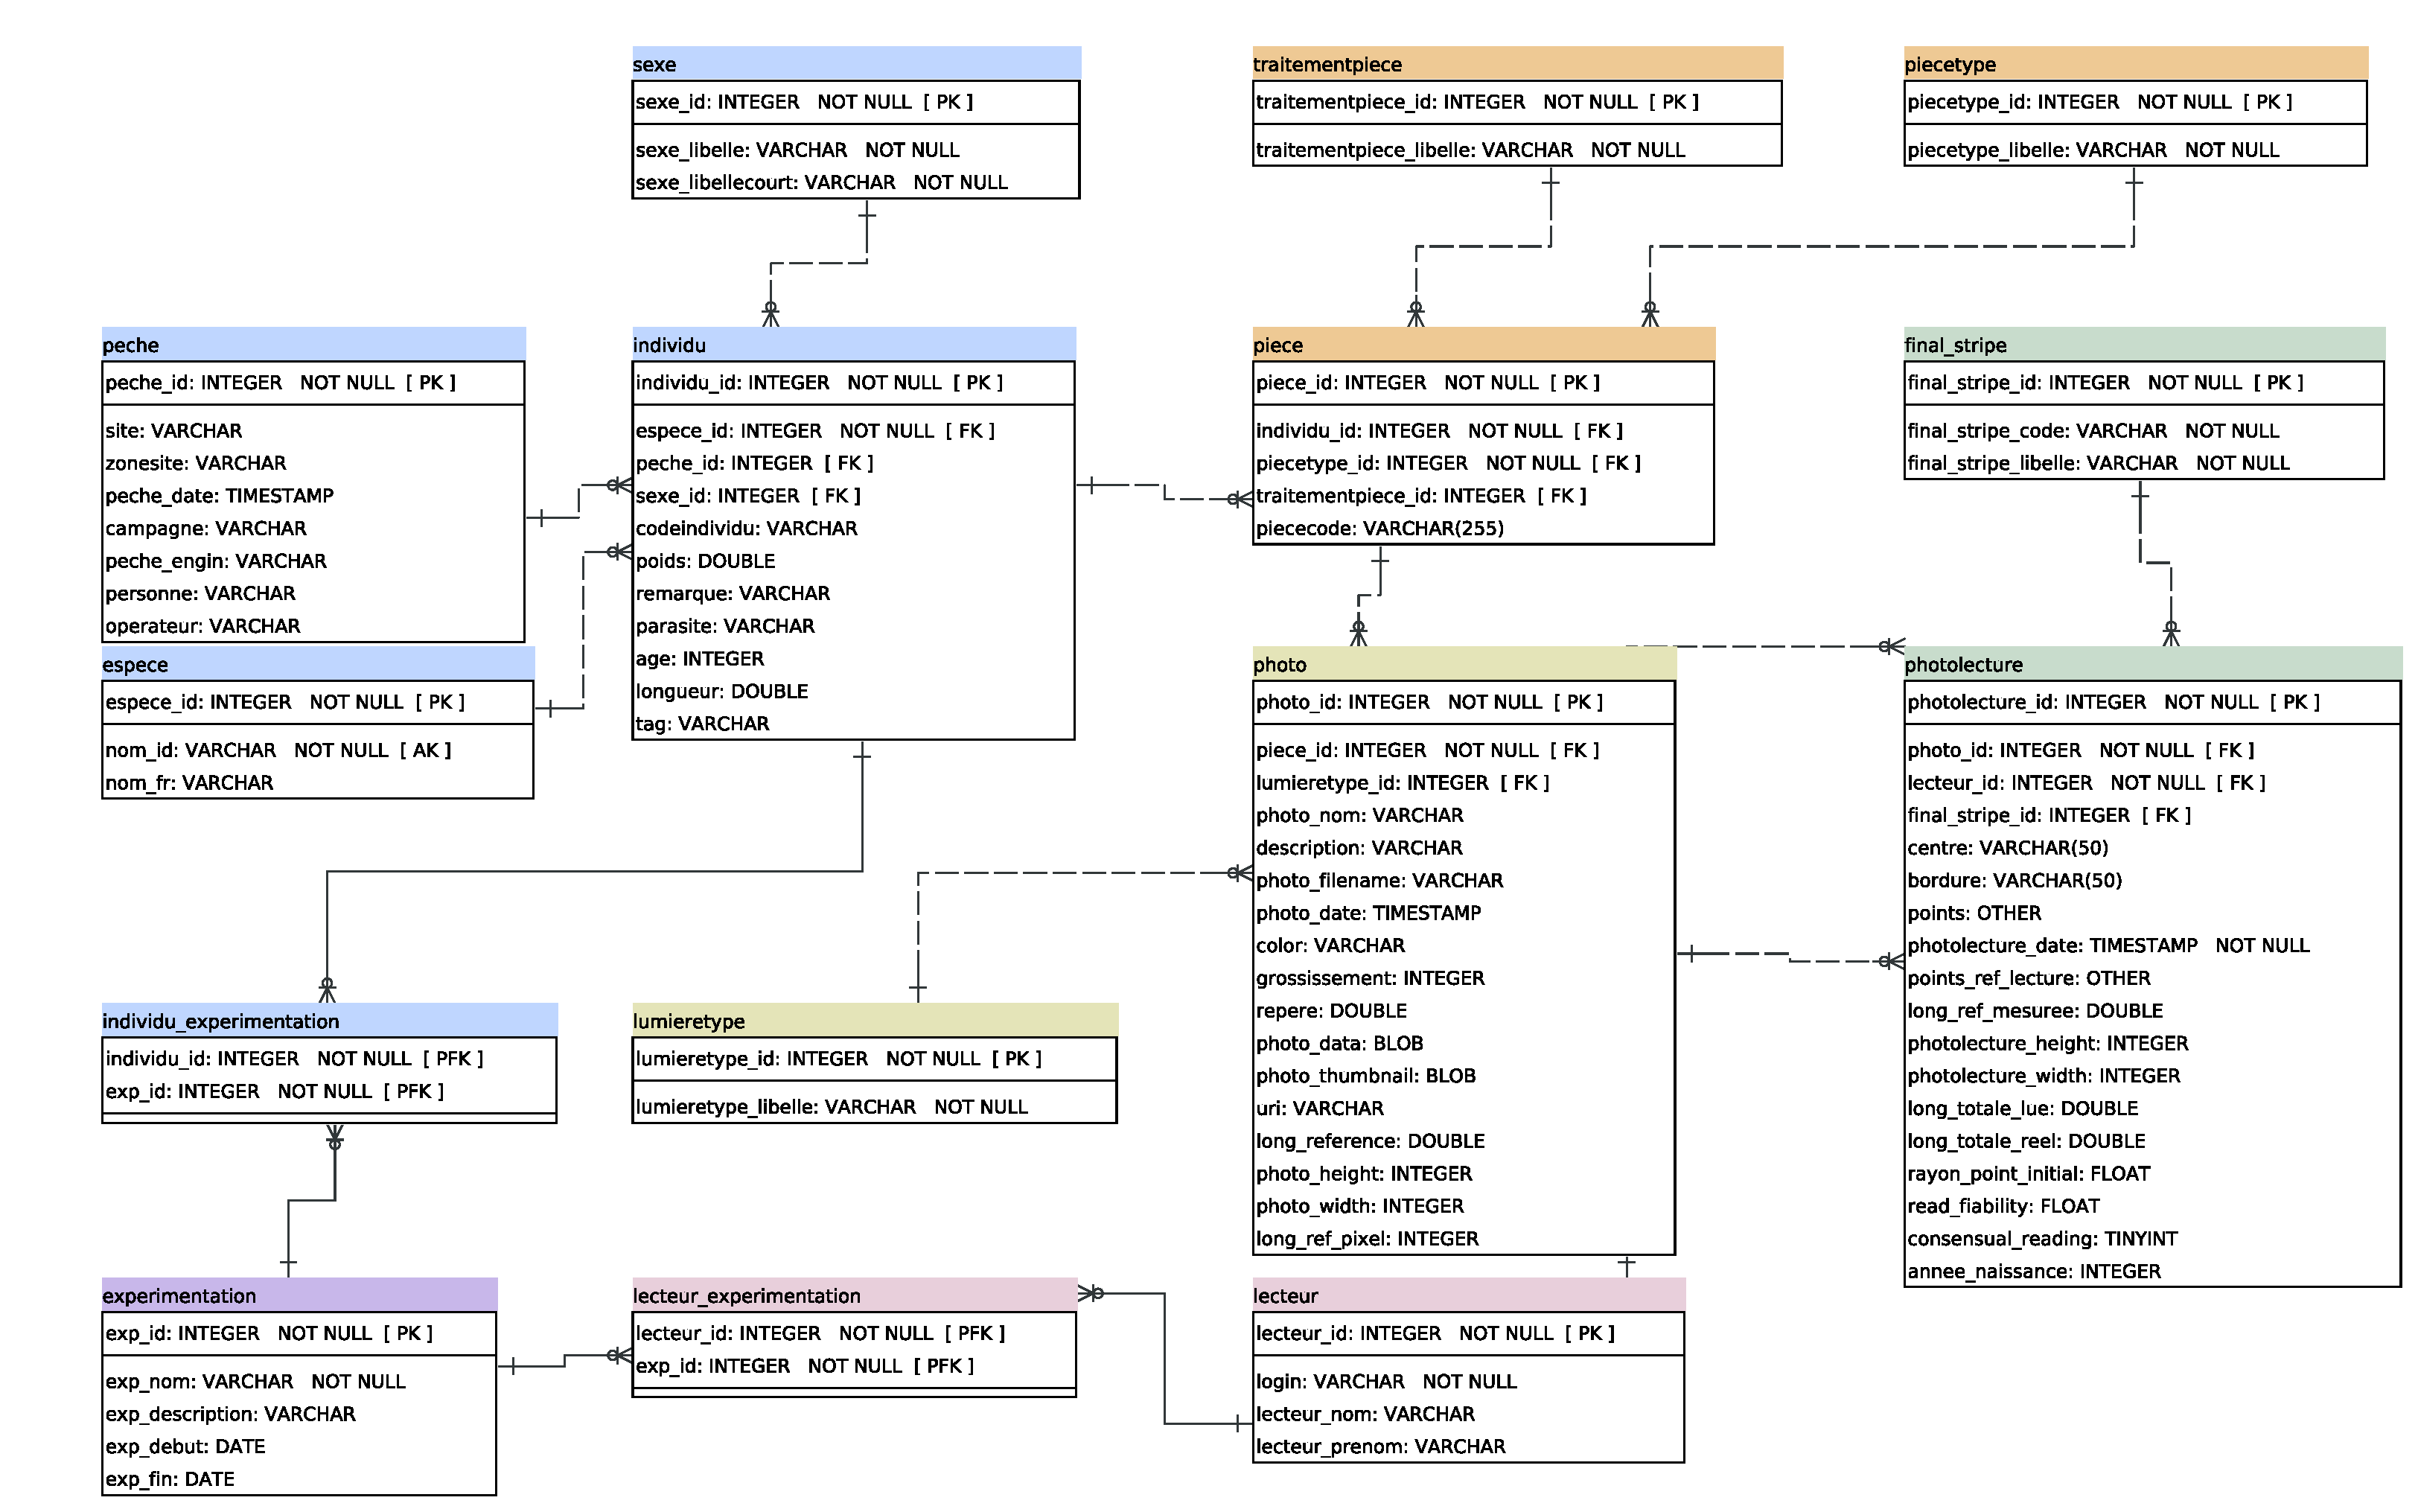
\includegraphics[width=\linewidth,angle=90]{db_schema}


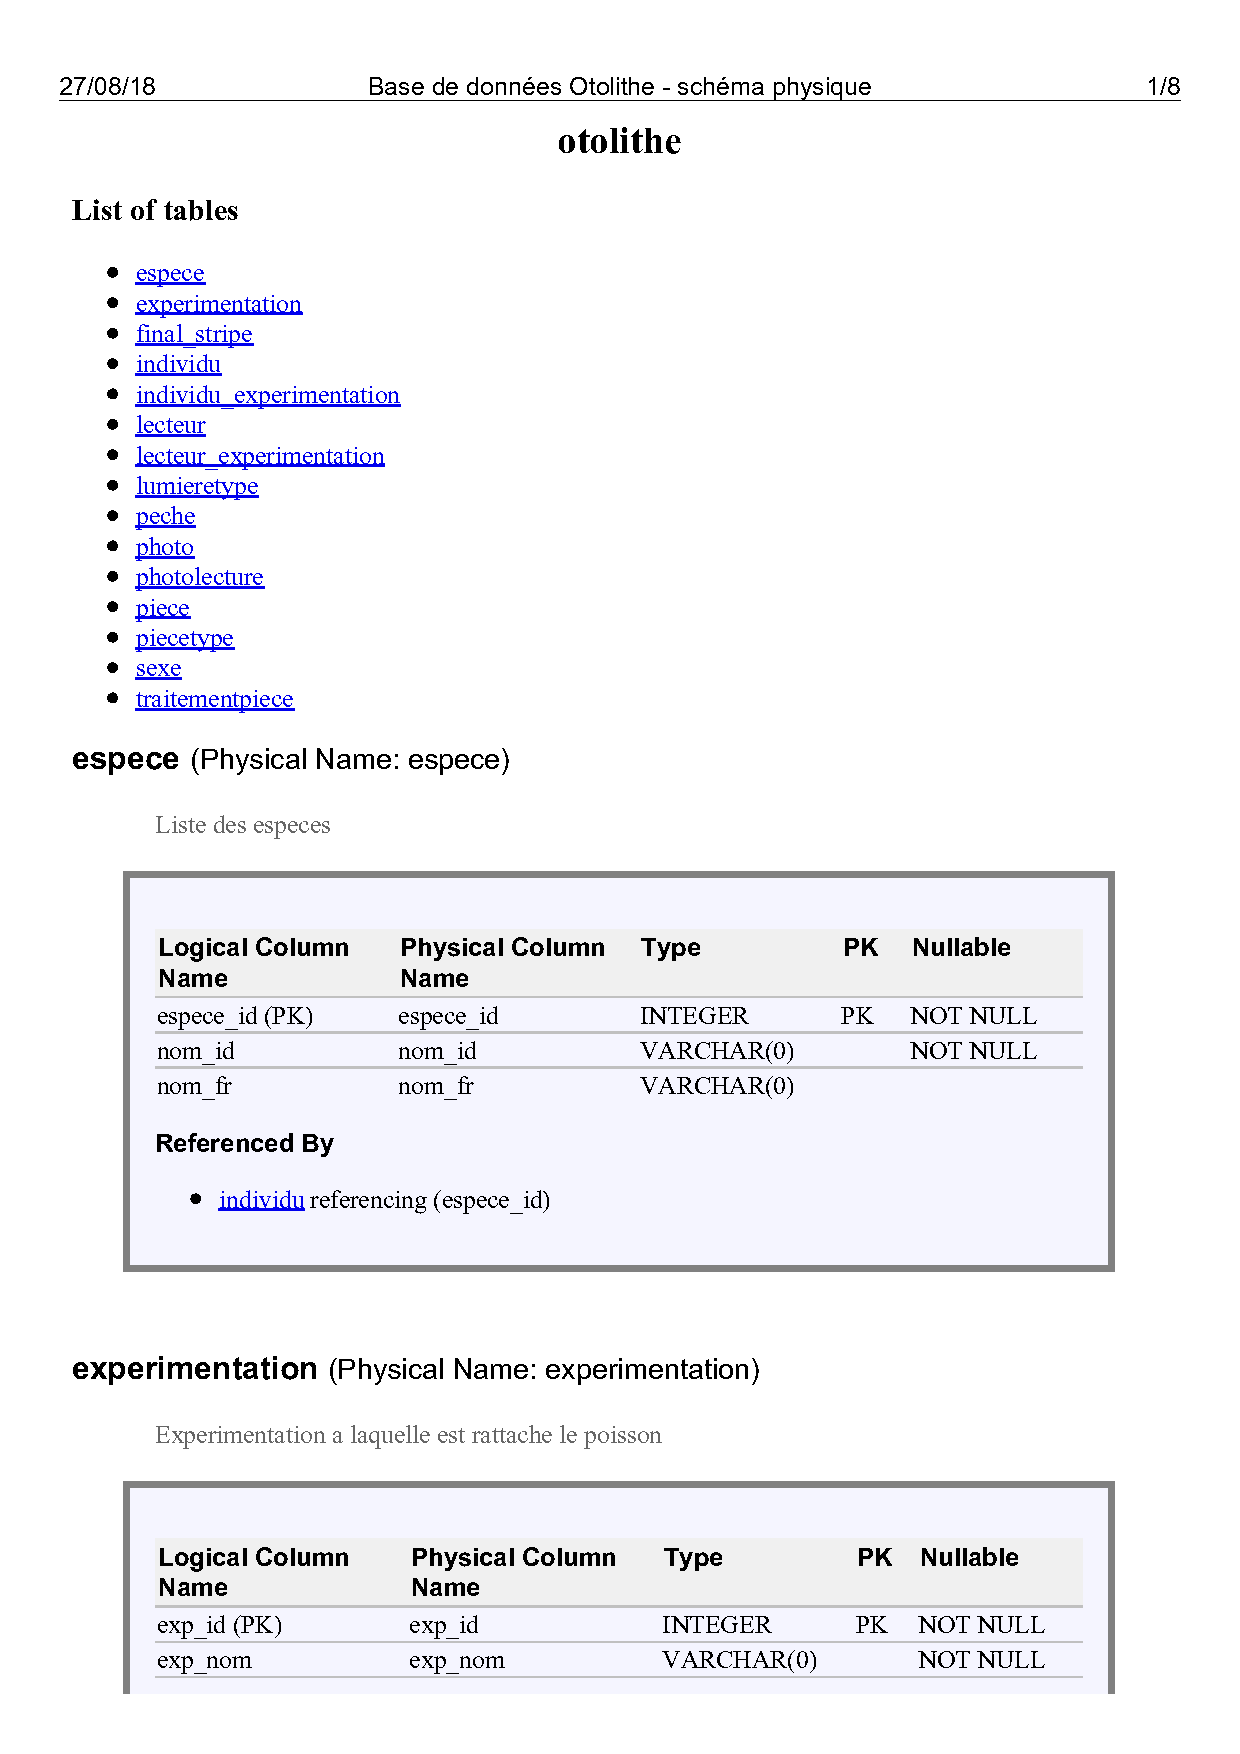
\includepdf[pages=1-8]{db_description.pdf}

%Bibliographie
\backmatter

% Integration de la biblio
% Pour insérer toutes les références : 
%\nocite{*}
% Pour intégrer une référence non citée : 
%\nocite{ref}
\nocite{*}
\bibliography{otolithe}

\end{document}